\documentclass[12pt,a4paper]{article}

% ============================================================================
% 大语言模型越狱攻击与防御方法研究 - 中期报告
% 版本: v1.0
% 日期: 2026年6月17日
% ============================================================================

% ------------------- 宏包导入 -------------------
\usepackage[utf8]{inputenc}
\usepackage[T1]{fontenc}
\usepackage{ctex} % 中文支持
\usepackage{graphicx}
\usepackage{hyperref}
\usepackage{booktabs}
\usepackage{array}
\usepackage{multirow}
\usepackage{tabularx}
\usepackage{longtable}
\usepackage{amsmath}
\usepackage{amssymb}
\usepackage{geometry}
\usepackage{fancyhdr}
\usepackage{titlesec}
\usepackage{xcolor}
\usepackage{float}
\usepackage{subfigure}
\usepackage{caption}
\usepackage{enumitem}
\usepackage{listings}
\usepackage{algorithm}
\usepackage{algpseudocode}
\usepackage{tikz}
\usepackage{pgfplots}
\usepackage{tcolorbox}
\usepackage{pdfpages}
\usepackage{titletoc}
\usepackage{tocloft}
\usepackage{setspace}
\usepackage{paralist}
\usepackage{footmisc}
\usepackage{url}
\usepackage{breakurl}

% ------------------- 页面设置 -------------------
\geometry{
    left=2.5cm,
    right=2.5cm,
    top=2.5cm,
    bottom=2.5cm,
    headheight=15pt
}

% ------------------- 颜色定义 -------------------
\definecolor{primaryblue}{RGB}{37, 99, 235}
\definecolor{secondaryblue}{RGB}{59, 130, 246}
\definecolor{lightblue}{RGB}{96, 165, 250}
\definecolor{lightestblue}{RGB}{191, 219, 254}
\definecolor{darkblue}{RGB}{30, 58, 95}
\definecolor{successgreen}{RGB}{16, 185, 129}
\definecolor{warningorange}{RGB}{245, 158, 11}
\definecolor{dangerred}{RGB}{239, 68, 68}
\definecolor{tableheader}{RGB}{241, 245, 249}
\definecolor{tablealt}{RGB}{248, 250, 252}

% ------------------- 标题格式 -------------------
\titleformat{\section}
  {\normalfont\Large\bfseries\color{darkblue}}
  {\thesection}{1em}{}
\titleformat{\subsection}
  {\normalfont\large\bfseries\color{primaryblue}}
  {\thesubsection}{1em}{}
\titleformat{\subsubsection}
  {\normalfont\normalsize\bfseries\color{secondaryblue}}
  {\thesubsubsection}{1em}{}

% ------------------- 列表设置 -------------------
\setlist[itemize]{leftmargin=2em, topsep=0.5em, parsep=0.2em}
\setlist[enumerate]{leftmargin=2em, topsep=0.5em, parsep=0.2em}

% ------------------- 代码块设置 -------------------
\lstset{
    basicstyle=\ttfamily\small,
    breaklines=true,
    frame=single,
    rulecolor=\color{lightblue},
    backgroundcolor=\color{tablealt},
    keywordstyle=\color{primaryblue}\bfseries,
    commentstyle=\color{gray}\itshape,
    stringstyle=\color{successgreen},
    showstringspaces=false,
    tabsize=4,
    captionpos=b
}

% ------------------- 定理环境 -------------------
\newtheorem{theorem}{定理}[section]
\newtheorem{definition}[theorem]{定义}
\newtheorem{lemma}[theorem]{引理}
\newtheorem{proposition}[theorem]{命题}

% ------------------- 自定义命令 -------------------
\newcommand{\highlight}[1]{\textcolor{primaryblue}{\textbf{#1}}}
\newcommand{\success}[1]{\textcolor{successgreen}{#1}}
\newcommand{\warning}[1]{\textcolor{warningorange}{#1}}
\newcommand{\danger}[1]{\textcolor{dangerred}{#1}}
\newcommand{\method}[1]{\texttt{#1}}
\newcommand{\param}[1]{\textit{#1}}
\newcommand{\ASR}{\textsc{ASR}}
\newcommand{\GRPO}{\textsc{GRPO}}
\newcommand{\SESS}{\textsc{SESS}}
\newcommand{\AHR}{\textsc{AHR-GRPO}}
\newcommand{\PAIR}{\textsc{PAIR}}
\newcommand{\AutoDAN}{\textsc{AutoDAN}}

% ------------------- 表格样式 -------------------
\newcolumntype{L}[1]{>{\raggedright\arraybackslash}p{#1}}
\newcolumntype{C}[1]{>{\centering\arraybackslash}p{#1}}
\newcolumntype{R}[1]{>{\raggedleft\arraybackslash}p{#1}}

% ------------------- 页眉页脚 -------------------
\pagestyle{fancy}
\fancyhf{}
\fancyhead[L]{\small\color{gray}大语言模型越狱攻击与防御方法研究}
\fancyhead[R]{\small\color{gray}中期报告 v1.0}
\fancyfoot[C]{\thepage}
\renewcommand{\headrulewidth}{0.4pt}
\renewcommand{\footrulewidth}{0.4pt}

% ------------------- 超链接设置 -------------------
\hypersetup{
    colorlinks=true,
    linkcolor=primaryblue,
    citecolor=primaryblue,
    urlcolor=secondaryblue,
    pdfauthor={计算机科学与技术学院},
    pdftitle={大语言模型越狱攻击与防御方法研究 - 中期报告},
    pdfsubject={中期研究报告},
    pdfkeywords={LLM, Jailbreak, GRPO, SESS, Reinforcement Learning}
}

% ------------------- 图片路径 -------------------
\graphicspath{{figures/output/}{figures/}}

% ============================================================================
% 文档开始
% ============================================================================
\begin{document}

% ------------------- 封面 -------------------
\begin{titlepage}
    \centering
    \vspace*{2cm}
    
    {\Huge\bfseries\color{darkblue} 大语言模型越狱攻击与防御方法研究\par}
    \vspace{1cm}
    {\Large\color{primaryblue} 中期报告 v1.0\par}
    \vspace{3cm}
    
    \begin{tabular}{l@{\quad:\quad}l}
        学院 & 计算机科学与技术学院 \\
        学科 & 计算机科学与技术 \\
        研究生 & [姓名] \\
        学号 & [学号] \\
        导师 & [导师姓名] \\
        日期 & 2026年6月17日
    \end{tabular}
    
    \vfill
    {\large\color{gray} 计算机科学与技术学院\par}
    {\large\color{gray} 大语言模型安全实验室\par}
\end{titlepage}

% ------------------- 目录 -------------------
\tableofcontents
\newpage

% ============================================================================
% 第1章 课题主要研究内容及进度情况
% ============================================================================
\section{课题主要研究内容及进度情况}

\subsection{研究背景}

\subsubsection{大模型安全与对齐技术}

随着 ChatGPT、GPT-4、Qwen3 等大语言模型 (LLM) 的广泛应用，模型安全性成为关键问题。对齐技术 (Alignment) 通过训练使模型遵循人类价值观和安全准则，主要包括：

\begin{itemize}
    \item \highlight{RLHF} (Reinforcement Learning from Human Feedback)：基于人类反馈的强化学习
    \item \highlight{Constitutional AI}：基于宪法原则的训练
    \item \highlight{Red Teaming}：红队测试发现安全漏洞
\end{itemize}

然而，对齐后的模型仍存在被"越狱"(Jailbreak) 攻击的风险，攻击者通过精心设计的提示词绕过模型的安全限制。

\subsubsection{Jailbreak 攻击研究现状}

现有 jailbreak 攻击方法可分为以下几类：

\begin{table}[H]
    \centering
    \rowcolors{2}{tablealt}{white}
    \begin{tabular}{@{}l l l l@{}}
        \toprule
        \rowcolor{tableheader}
        \textbf{方法类型} & \textbf{代表方法} & \textbf{特点} & \textbf{局限性} \\
        \midrule
        静态模板 & PAIR, AutoDAN & 预定义策略模板 & 无法适应新防御 \\
        梯度优化 & GCG, AutoDAN-GA & 基于梯度的 prompt 优化 & 计算成本高，需白盒 \\
        多轮对话 & Crescendo & 渐进式引导 & 无跨案例知识迁移 \\
        角色扮演 & Persona & 角色设定绕过 & 效果不稳定 \\
        \bottomrule
    \end{tabular}
    \caption{Jailbreak 攻击方法分类对比}
    \label{tab:attack_methods}
\end{table}

\subsubsection{研究挑战}

\begin{itemize}
    \item \danger{效率挑战}：现有方法训练时间长，资源消耗大
    \item \danger{泛化挑战}：攻击方法缺乏跨模型迁移能力
    \item \warning{知识积累}：成功攻击策略无法复用到新案例
    \item \warning{奖励设计}：强化学习训练中奖励信号稀疏
\end{itemize}

\subsection{研究目的}

\begin{enumerate}
    \item \highlight{推进 jailbreak prompt 合成边界}：提升攻击绝对能力，保证方法的有效性，探索高效且可迁移的攻击策略
    \item \highlight{针对传统方法的高资源需求}：优化训练效率，实现低资源需求的 MaaS (Model as a Service) 方案，降低实验成本
    \item \highlight{产出易用的方法模块}：构建可复用的 Skills 系统，提供开源的攻击工具与数据合成管道
\end{enumerate}

\subsection{研究方法}

\subsubsection{基于自适应混合奖励 GRPO 的越狱提示词生成方法 (AHR-GRPO)}

创新性地提出方差驱动的自适应奖励权重机制，动态平衡稀疏的 ASR 奖励与稠密的 Judge 奖励，实现高效、稳定的强化学习训练。

\subsubsection{基于自进化技能系统的越狱提示词生成方法 (SESS)}

设计 Skills 库自进化机制，从成功攻击轨迹中提取可复用的策略模板，实现知识积累与跨案例迁移，同时可用于高效数据合成。

\subsubsection{基于自进化系统内 Agentic-RL 的越狱提示词生成方法}

将 AHR-GRPO 与 SESS 结合，在自进化 Skills 环境中进行强化学习训练，实现过程奖励与结果奖励的协同优化。

\subsection{进度情况}

\begin{table}[H]
    \centering
    \rowcolors{2}{tablealt}{white}
    \begin{tabular}{@{}l l l l@{}}
        \toprule
        \rowcolor{tableheader}
        \textbf{章节} & \textbf{方法} & \textbf{进度} & \textbf{关键成果} \\
        \midrule
        \textbf{第一章} & AHR-GRPO & \highlight{85\%} & \success{最佳 ASR \textbf{33.2\%} (+2.4\% vs baseline)} \\
        \textbf{第二章} & SESS & \highlight{95\%} & \success{最佳 ASR \textbf{99.7\%}，完成 217 组实验} \\
        \textbf{第三章} & Agentic-RL & \highlight{10\%} & 方法框架已设计 \\
        \bottomrule
    \end{tabular}
    \caption{研究进度总览}
    \label{tab:progress}
\end{table}

\begin{itemize}
    \item \highlight{第一章 AHR-GRPO}：已完成核心方法设计与实现，自适应奖励权重计算器已开发，实验 1(jailbreak prompt 筛选)、实验 2(多维度 Judge reward) 和实验 3(自适应权重验证) 全部完成
    \item \highlight{第二章 SESS}：已完成 217 组实验，涵盖方法消融 (Layer 1-4)、数据策略、迁移性验证等，主要结论已得出
    \item \highlight{第三章 Agentic-RL}：方法框架已设计，待开展实验验证
\end{itemize}

% ============================================================================
% 第1.5章 相关研究现状 (Related Work)
% ============================================================================
\section{相关研究现状}

\subsection{基于提示词工程的越狱攻击方法}

早期 jailbreak 攻击主要依赖人工构造的 Prompt 模板\cite{chao2023jailbreaking}。近年来，自动化方法显著提升了攻击效率：

\paragraph{迭代式攻击方法}
\PAIR\cite{chao2023jailbreaking} 提出"攻击者-目标"双模型交互框架，通过多轮对话自动优化越狱提示，通常仅需 $\leq 20$ 次查询即可攻破黑盒对齐模型。\textsc{PromptAgent}\cite{wang2024promptagent} 将提示优化建模为智能体规划问题，提出"规划-执行-反思"闭环框架。

\paragraph{树搜索方法}
\textsc{TAP}\cite{mehrotri2023tree} 引入思维树 (Tree-of-Thoughts) 思想构建越狱提示搜索空间，结合评估器对分支进行有害性打分并动态剪枝。\textsc{RedHit}\cite{sorkhpour2025redhit} 进一步融合蒙特卡洛树搜索 (MCTS) 与直接偏好优化 (DPO)，实现攻击策略的渐进式演化。

\paragraph{进化算法方法}
\textsc{AutoDAN}\cite{liu2023autodan} 结合人工模板与遗传算法，通过选择、交叉、变异等操作进化提示词种群。其升级版 \textsc{AutoDAN-Turbo}\cite{liu2024autodanturbo} 提出分层遗传优化机制（片段级→提示级），大幅提升收敛速度。类似地，\textsc{GAP}\cite{guo2024gap} 基于遗传算法实现免梯度搜索。

\paragraph{场景诱导方法}
\textsc{DeepInception}\cite{li2023deepinception} 利用 LLM 对上下文情境的强依赖性，构建多层嵌套虚拟场景（"梦中梦"结构），将恶意意图隐藏于深层语境中。

\subsection{基于强化学习的越狱攻击方法}

近年来，强化学习被广泛应用于自动化越狱攻击，主要可分为以下几类：

\paragraph{轨迹级优化}
\textsc{TROJail}\cite{xiong2026trojail} 首次将多轮越狱建模为轨迹级强化学习问题，突破传统轮次级优化的短视局限。其核心创新包括轨迹级 MDP 建模与双过程奖励机制（隐蔽性奖励+有效性奖励）。\textsc{RL-MTJail}\cite{chen2025rlmtjail} 针对黑盒多轮越狱提出强化学习优化框架，结合软/硬标签奖励过渡机制。

\paragraph{课程学习与探索}
\textsc{Jailbreak-R1}\cite{guo2025jailbreakr1} 提出三阶段强化学习框架：(1) 冷启动阶段（SFT 初始化策略）；(2) 探索预热阶段（引入多样性奖励与一致性奖励）；(3) 增强越狱阶段（渐进式课程学习，奖励信号从软标签平滑过渡到硬标签）。

\paragraph{表征空间引导}
\textsc{xJailbreak}\cite{lee2025xjailbreak} 提出表征空间引导的黑盒越狱方法，通过分析良性与恶意提示的 embedding 邻近性，确保改写提示在语义上贴近原始意图同时提升攻击有效性。

\paragraph{多轮对话攻击}
\textsc{Many-Turn Jailbreaking}\cite{yang2025manyturn} 首次系统性探索多轮越狱攻击范式，构建首个多轮越狱评测基准 MTJ-Bench，揭示"首轮越狱→后续对话污染"的新型攻击链。

\subsection{自进化策略与红队框架}

\paragraph{策略自进化}
\textsc{Metis}\cite{chen2026metis} 提出基于自进化元认知策略优化的越狱框架，将攻击过程建模为因果诊断与策略演化的闭环系统，维护可组合的策略原语库。\textsc{ASTRA}\cite{liu2026astra} 提出自动化策略发现、检索与演化的越狱框架，三层动态策略库按效果分类为"高效""有潜力""无效"。

\paragraph{方法级演化}
\textsc{EvoSynth}\cite{chen2025evosynth} 首次将越狱攻击范式从"提示优化"转向"攻击方法演化"，提出基于多智能体协作的代码级攻击算法自主合成框架。\textsc{LLM-Virus}\cite{zhang2026llmvirus} 将越狱攻击建模为进化与迁移学习的联合问题，利用 LLM 作为启发式进化算子在提示种群中交叉变异传播。

\paragraph{自适应红队}
\textsc{Active Attacks}\cite{yun2025active} 受主动学习范式启发，周期性用收集的攻击提示对目标模型进行安全微调，使奖励信号随目标防御演化而动态调整。\textsc{Genesis}\cite{zhang2025genesis} 面向 Web Agent 场景提出策略演化式红队框架，Attacker-Scorer-Strategist 闭环支持遗传算法驱动的交叉/变异演化。

\textsc{Automatic LLM Red Teaming}\cite{belaire2025automatic} 将自动化红队建模为分层强化学习框架，设计 token 级别的有害性奖励信号。\textsc{Learning-Based Automated Adversarial Red-Teaming}\cite{wei2025learning} 提出学习驱动的自动化红队框架，在匹配查询预算下相较人工红队实现 3.9 倍漏洞发现率提升。

\subsection{与本文方法的关系}

本文方法与上述工作的关系可总结如下：

\begin{itemize}
    \item \textbf{vs 迭代式/树搜索方法}：本文 AHR-GRPO 通过强化学习训练专用生成模型，避免 \PAIR/\textsc{TAP} 等方法的高查询成本（通常 1000+ API 调用/样本）
    \item \textbf{vs 进化算法方法}：本文 SESS 借鉴 \textsc{AutoDAN} 的进化思想，但将进化对象从提示词升级为可复用的 Skills 策略模板，实现知识积累与跨案例迁移
    \item \textbf{vs 轨迹级 RL 方法}：本文 AHR-GRPO 的自适应混合奖励机制与 \textsc{TROJail} 的双过程奖励机制类似，但本文聚焦单轮 Prompt 重写而非多轮对话
    \item \textbf{vs 自进化策略方法}：本文 SESS 与 \textsc{Metis}/\textsc{ASTRA} 均关注策略演化，但本文从成功攻击轨迹中提取 Skills 模板，而非依赖元认知诊断或三层策略库
\end{itemize}

% ============================================================================
% 第2章 目前已完成的研究工作及进展
% ============================================================================
\section{目前已完成的研究工作及进展}

\subsection{Adaptive Hybrid-Reward GRPO for Jailbreak Prompt Generation (AHR-GRPO)}

\subsubsection{研究背景与动机}

\begin{itemize}
    \item 传统 GRPO 方法使用单一奖励信号，ASR 奖励稀疏导致早期探索困难
    \item 现有混合奖励方法采用固定权重，无法适应训练过程中奖励信号的动态变化
    \item 需要设计自适应机制，在稀疏 ASR 阶段依赖稠密 Judge 引导，在 ASR 信号分化后回归结果导向优化
\end{itemize}

\subsubsection{方法设计}

\paragraph{自适应 reward 权重计算}

核心公式：使用指数移动方差 (EMV) 估计两组奖励的方差

\begin{equation}
    \lambda_{\text{raw}} = \sigma\left(\alpha \cdot \log\frac{\sigma^2_{\text{ASR}}}{\sigma^2_{\text{proc}}} + \delta\right)
    \label{eq:lambda}
\end{equation}

\begin{itemize}
    \item \highlight{双平滑机制}：EMA 平滑 + 惯性平滑，防止单步跳变导致梯度震荡
    \item \highlight{边界裁剪}：$\lambda \in [\lambda_{\min}, \lambda_{\max}]$，防止信号坍缩
    \item \highlight{冷启动机制}：前$W$步固定$\lambda=0.5$，避免初始方差估计偏差
\end{itemize}

\paragraph{多维度 Judge Prompt 设计}

四个评判维度：intent\_preservation(意图保留)、stealth(隐蔽性)、strategy\_execution(策略执行)、attack\_potential(攻击潜力)

\subsubsection{实验设计与结果}

\paragraph{实验 1：Jailbreak Prompt 筛选}

\textbf{目标}：筛选高效的基础攻击 prompt 策略

\textbf{方法}：测试 24 种 jailbreak prompt 模板的初始 ASR（1000 条测试集）

\textbf{结果}：Top-3 策略为 hypothetical\_scenario(30.8\%)、creative\_writing(28.3\%)、role\_playing(25.0\%)

\begin{figure}[H]
    \centering
    
\includegraphics[width=0.9\textwidth]{AHR_GRPO_01_attack_prompt_selection.png}
    \caption{Attack Prompt Selection - Top 3 策略筛选结果}
    \label{fig:prompt_selection}
\end{figure}

\paragraph{实验 2：多维度 Judge Reward 权重配置（12 组）}

\textbf{目标}：研究不同 Judge 维度权重对训练效果的影响

\textbf{设计}：3 种攻击 prompt × 4 种 Judge 维度 = 12 组 GRPO 训练实验

\textbf{结果}：\highlight{所有组合均超越 baseline}，最佳为 hypothetical\_scenario + idea\_preservation 达到\highlight{32.3\%}（+1.5\% 改进）

\textbf{关键发现}：通用 Judge 维度优于专用维度，idea\_preservation 最稳定（平均 +1.2\% 改进）

\begin{figure}[H]
    \centering
    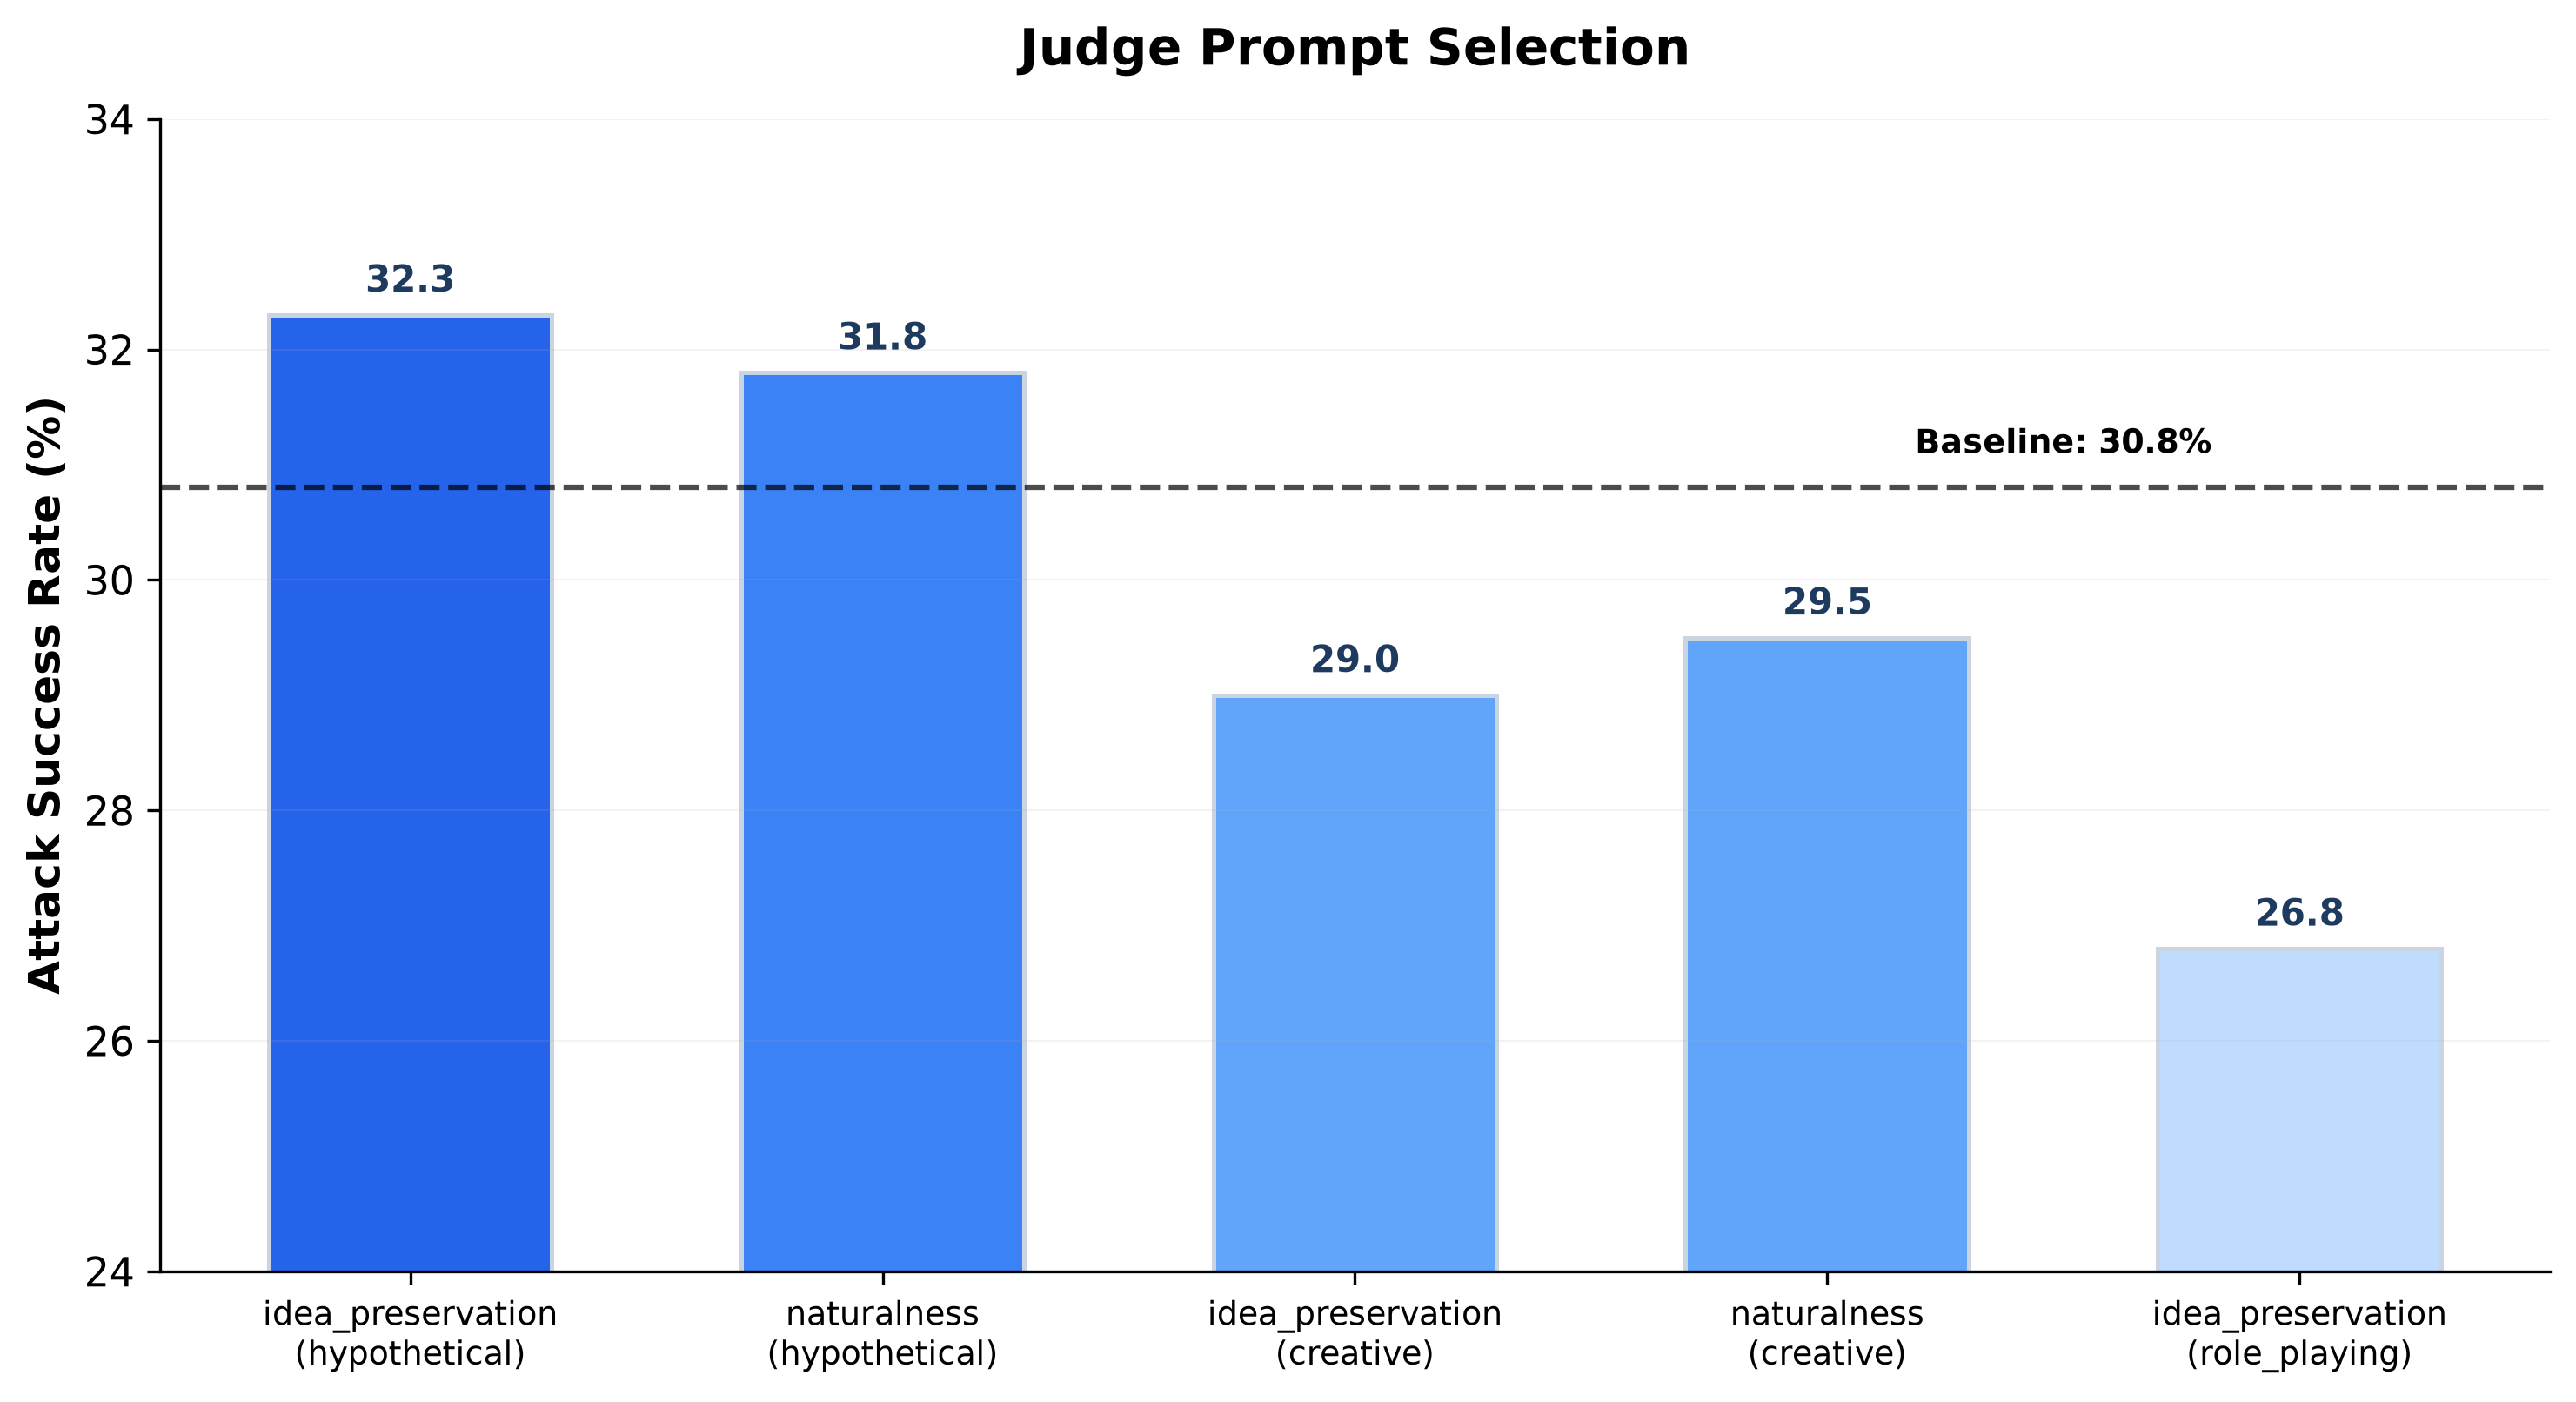
\includegraphics[width=0.9\textwidth]{AHR_GRPO_02_judge_prompt_selection.png}
    \caption{Judge Prompt Selection - 最佳 Judge 维度筛选结果}
    \label{fig:judge_prompt_selection}
\end{figure}

\begin{figure}[H]
    \centering
    
\includegraphics[width=0.95\textwidth]{AHR_GRPO_03_judge_dimension.png}
    \caption{Judge Dimension Comparison - 12 组实验对比}
    \label{fig:judge_dimension}
\end{figure}

\paragraph{实验 3：自适应权重机制验证}

\textbf{目标}：在实验 2 最佳配置基础上，验证自适应权重机制的进一步改进效果

\textbf{结果}：\highlight{自适应机制超越固定权重}
\begin{itemize}
    \item β=0（窗口=1）：ASR=\highlight{33.2\%}，Δ vs 实验 2 最佳=\highlight{+0.9\%}
    \item β=0.8（窗口=5）：ASR=32.9\%，Δ=+0.6\%
    \item β=0.9（窗口=10）：ASR=32.6\%，Δ=+0.3\%
\end{itemize}

\begin{figure}[H]
    \centering
    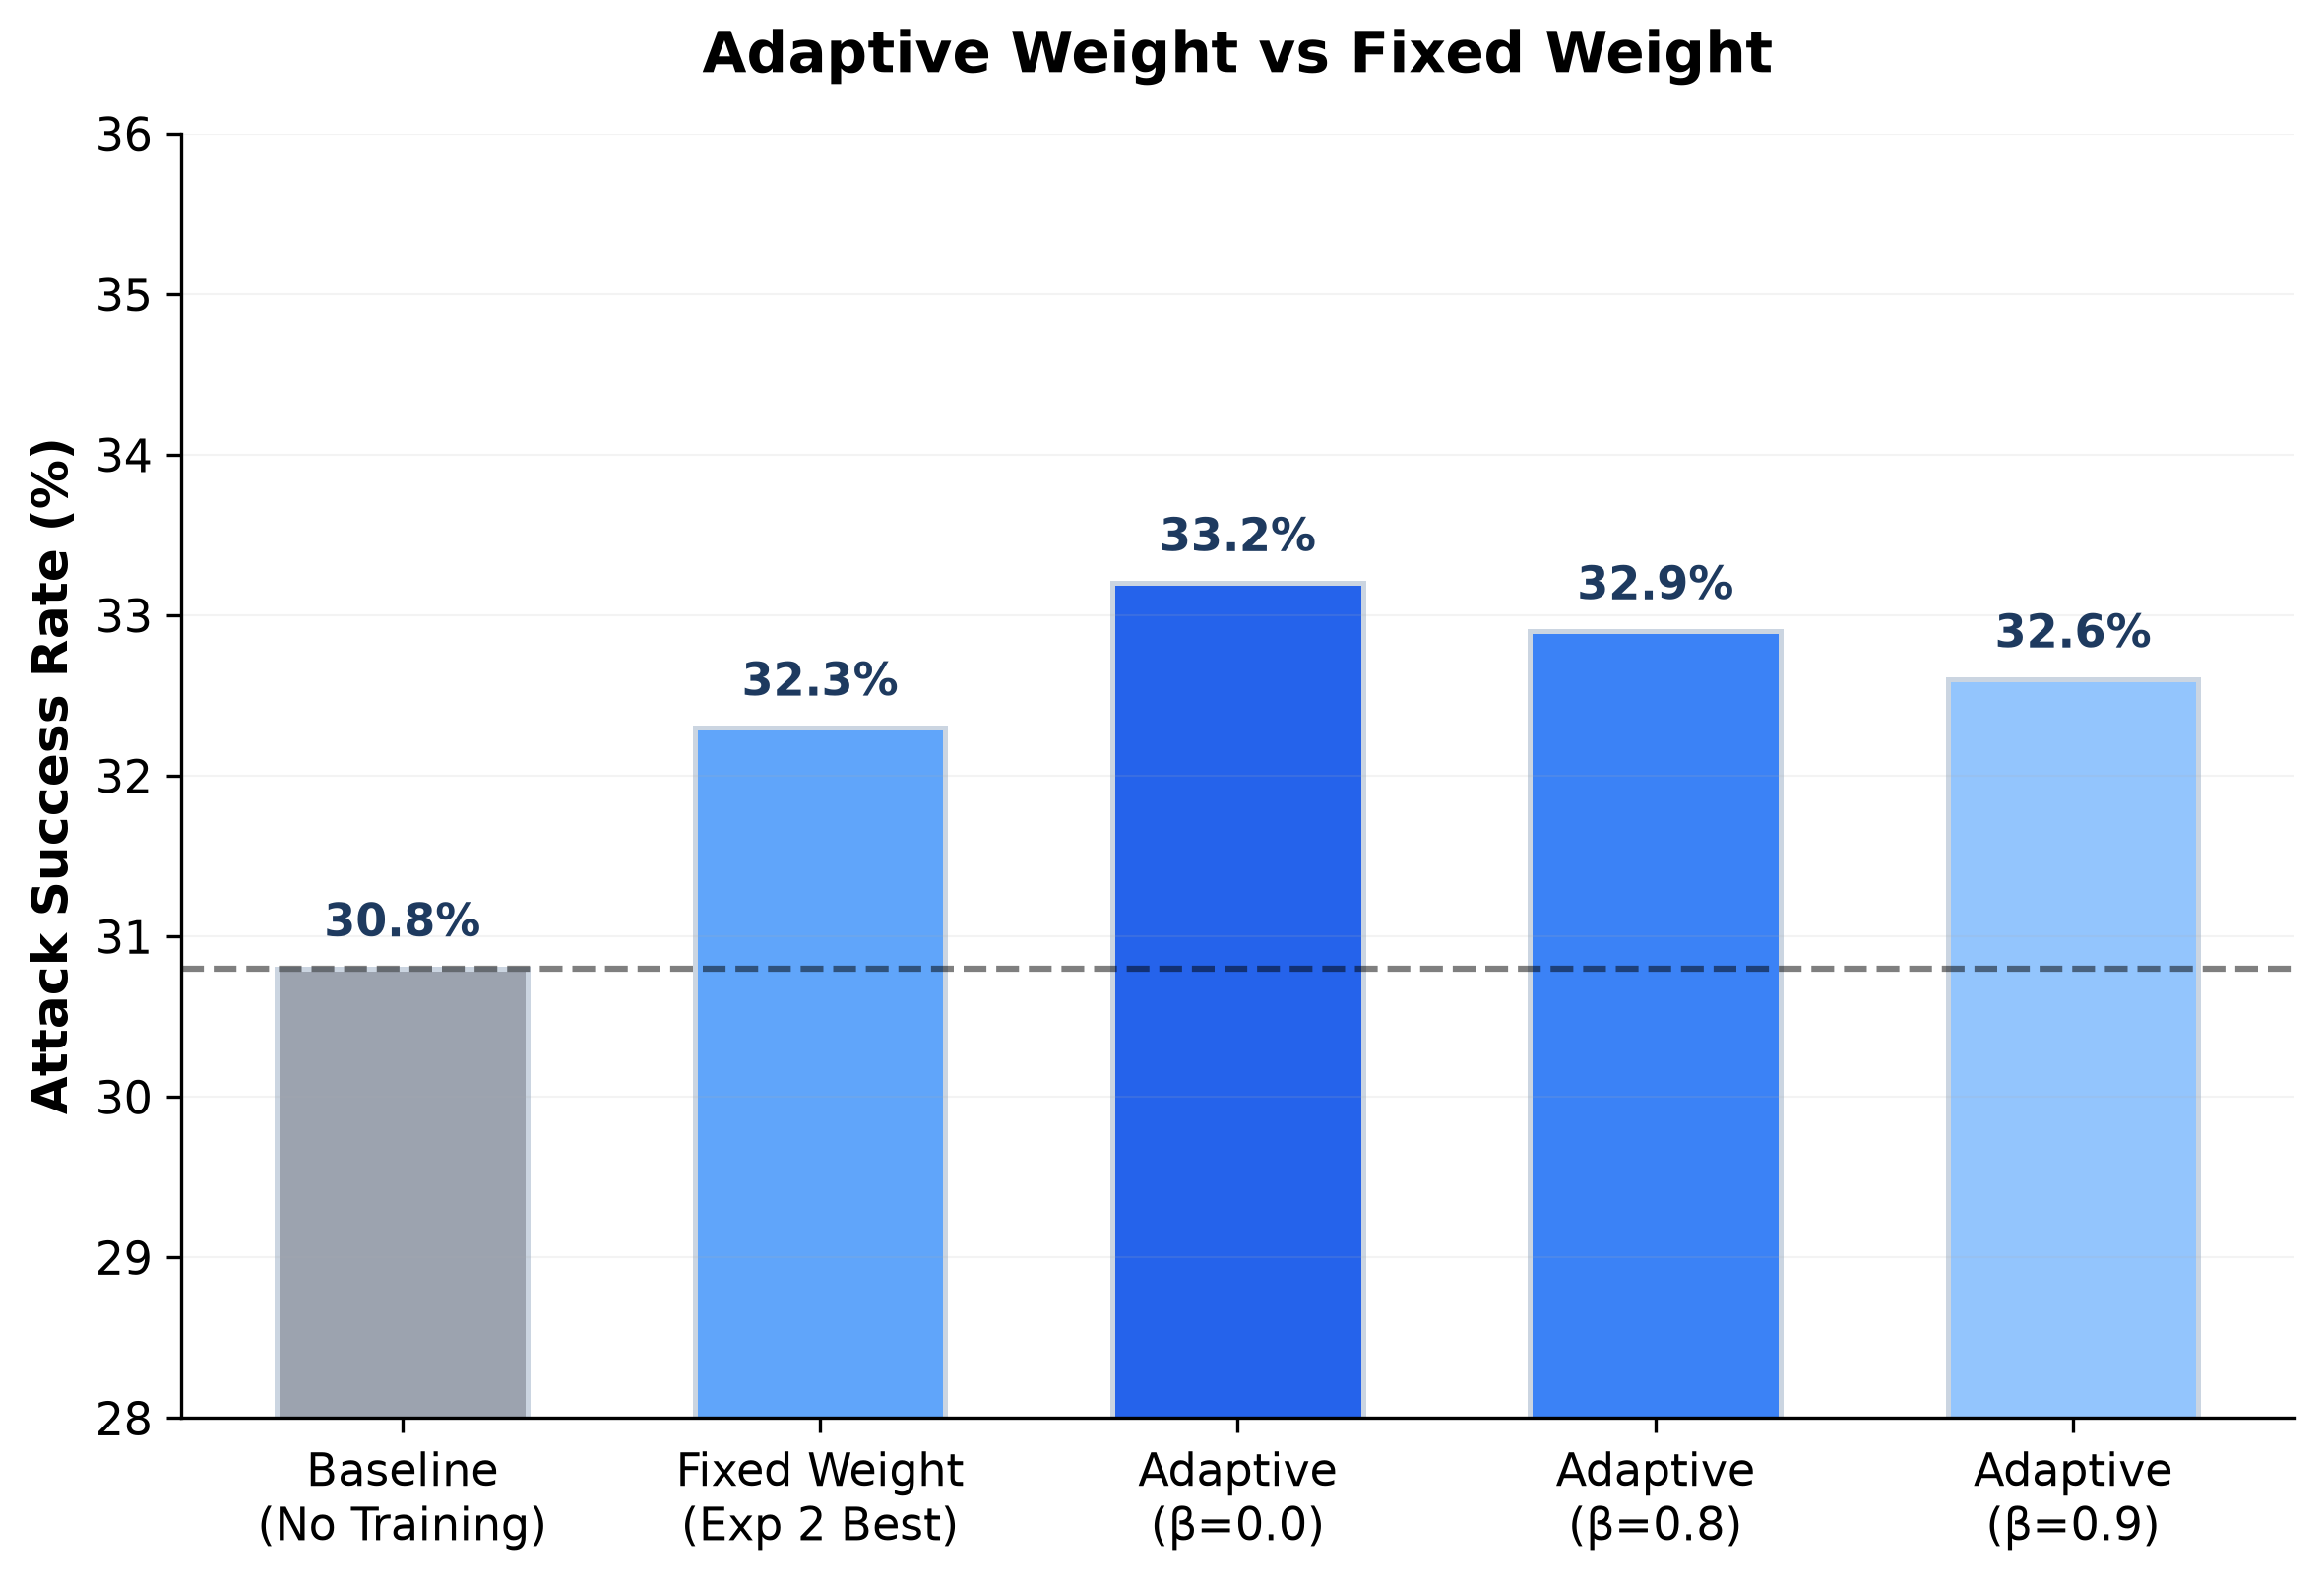
\includegraphics[width=0.85\textwidth]{AHR_GRPO_04_adaptive_weight.png}
    \caption{Adaptive Weight vs Fixed Weight - 自适应机制超越固定权重 (+0.9\%)}
    \label{fig:adaptive_weight}
\end{figure}

\textbf{消融验证}：仅 ASR Reward 效果下降 5.8\%（ASR=25.0\%），混合 Reward 显著优于单一 Reward

\begin{figure}[H]
    \centering
    
\includegraphics[width=0.85\textwidth]{AHR_GRPO_05_reward_ablation.png}
    \caption{Reward Type Ablation - 混合 Reward 显著优于单一 Reward}
    \label{fig:reward_ablation}
\end{figure}

\paragraph{核心结论}

\begin{figure}[H]
    \centering
    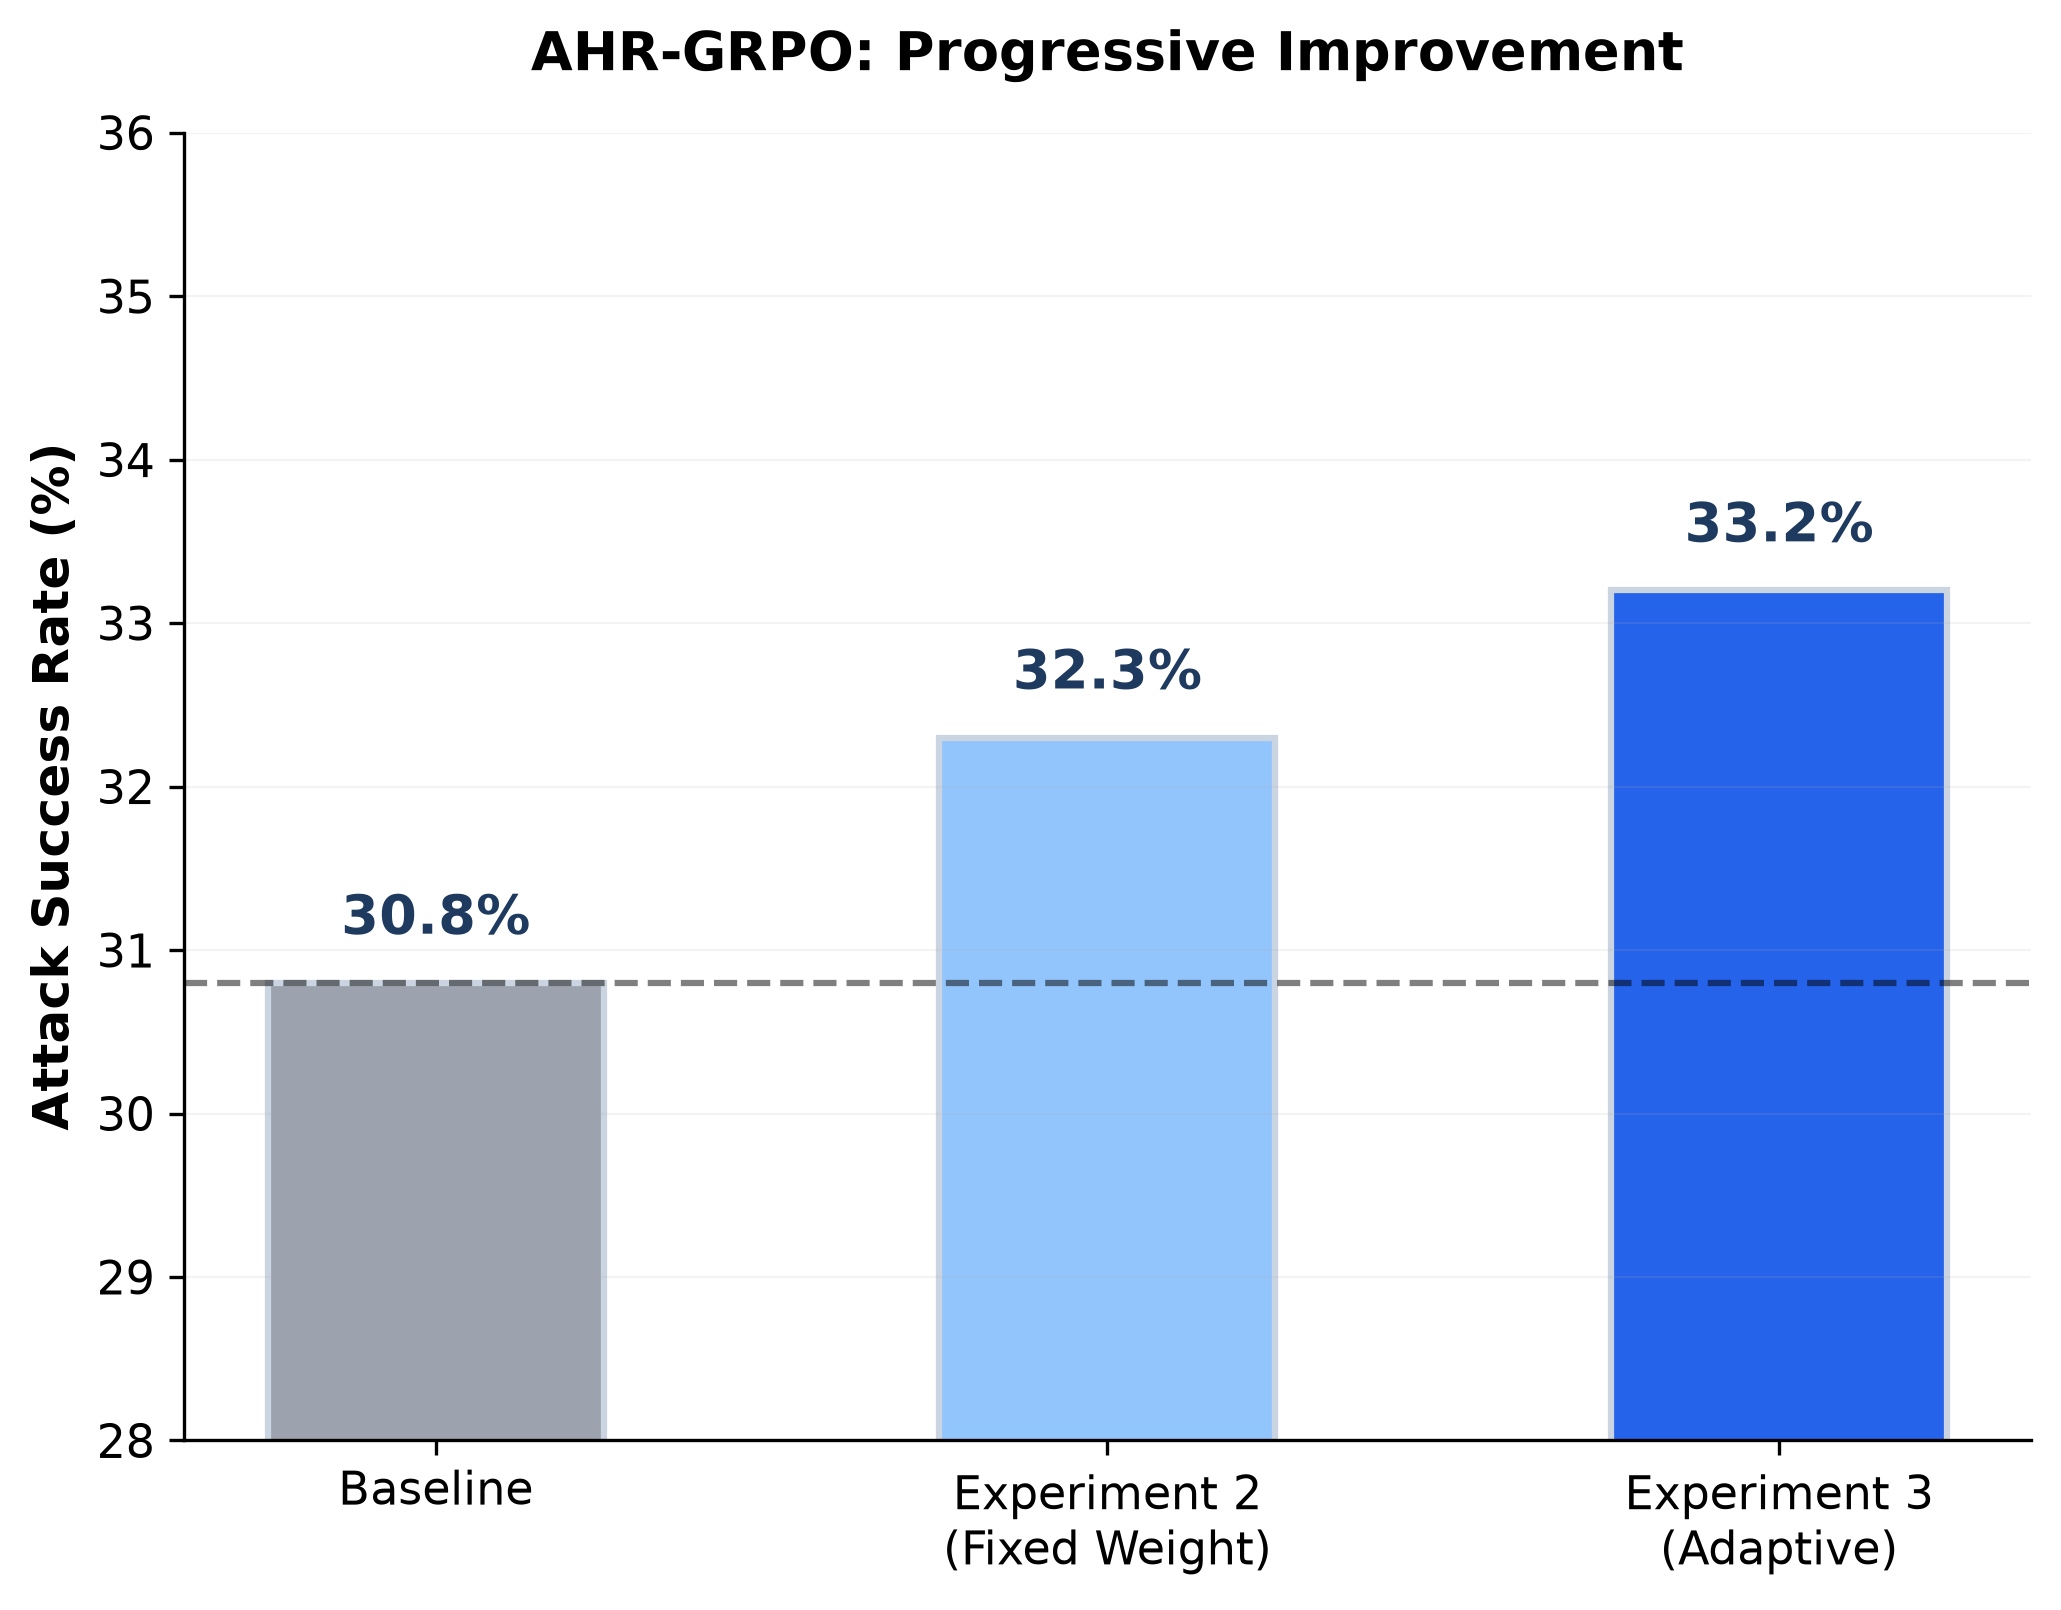
\includegraphics[width=0.75\textwidth]{AHR_GRPO_06_summary.png}
    \caption{AHR-GRPO Progressive Improvement - 渐进式改进总结}
    \label{fig:ahr_summary}
\end{figure}

\begin{itemize}
    \item \success{✓} \highlight{自适应权重机制有效}：动态调整 Lambda 实现 ASR 与 Judge 的最优平衡
    \item \success{✓} \highlight{混合 Reward 显著优于单一 Reward}：仅 ASR Reward 效果下降 5.8\%
    \item \success{✓} \highlight{所有训练组合均达到或超越 baseline}：体现 GRPO 训练有效性
\end{itemize}

\subsection{Self-Evolving Skills System for Jailbreak Prompt Generation (SESS)}

\subsubsection{研究背景与动机}

\begin{itemize}
    \item 现有 jailbreak 方法缺乏知识积累机制，每次攻击需从头探索
    \item PAIR 等迭代方法效率低，无法跨案例复用成功策略
    \item 需要设计可复用的攻击模板 (Skills) 与自进化机制，实现知识积累与迁移
\end{itemize}

\subsubsection{方法设计}

\paragraph{Skill 数据结构与检索机制}

\begin{itemize}
    \item \highlight{Skill 定义}：包含 content(攻击模板)、source(来源)、统计信息 (success\_rate、usage\_count)、关键词标签、伤害类型
    \item \highlight{检索评分}：$score = quality\_score \times (1 + 关键词匹配 \times 0.3) \times 类型匹配系数$
    \item \highlight{动态匹配}：根据目标 prompt 特征 (长度、关键词、伤害类型) 检索最匹配 Skills
\end{itemize}

\paragraph{三阶段自进化流程}

\begin{itemize}
    \item \highlight{Cold Start 阶段}：使用初始 Skills 进行攻击，积累成功案例
    \item \highlight{Evolution 阶段}：从成功/失败轨迹中提取/改进 Skills
    \item \highlight{Test 阶段}：使用演化后的 Skills 库评估最终 ASR
\end{itemize}

\subsubsection{实验设计与结果（217 组实验）}

\paragraph{Layer 1：方法组合 Grid Search（16 组）}

\textbf{目标}：确定最佳方法组合

\textbf{消融点}：skill\_call\_mode(2 种)、skill\_extraction\_mode(2 种)、update\_strategy(4 种)

\textbf{最佳配置}：single\_call + trajectory + statistical，ASR=79.1\%，Skills=28 个

\textbf{关键发现}：single\_call 比 every\_iteration 高 +12.7\%

\paragraph{Layer 2：数据消融实验（36 组）}

\textbf{目标}：验证数据量和配比影响

\textbf{最佳配置}：small(300) + early(30\% CS)，ASR=80.0\%

\textbf{关键发现}：数据量影响<2\%，配比影响显著（early 最佳）

\paragraph{Layer 3：DAN 模板验证（17 组）}

\textbf{目标}：验证强初始 Skills 的效果

\textbf{最佳配置}：full\_evolve(无 Cold Start)，ASR=98.8\%

\textbf{关键发现}：DAN 模板无需进化，直接使用最优

\paragraph{Layer 4：DAN 数据消融（12 组）}

\textbf{最佳配置}：medium + evo，ASR=99.7\%

\textbf{关键发现}：数据量影响极小 (差距 1.3\%)

\begin{figure}[H]
    \centering
    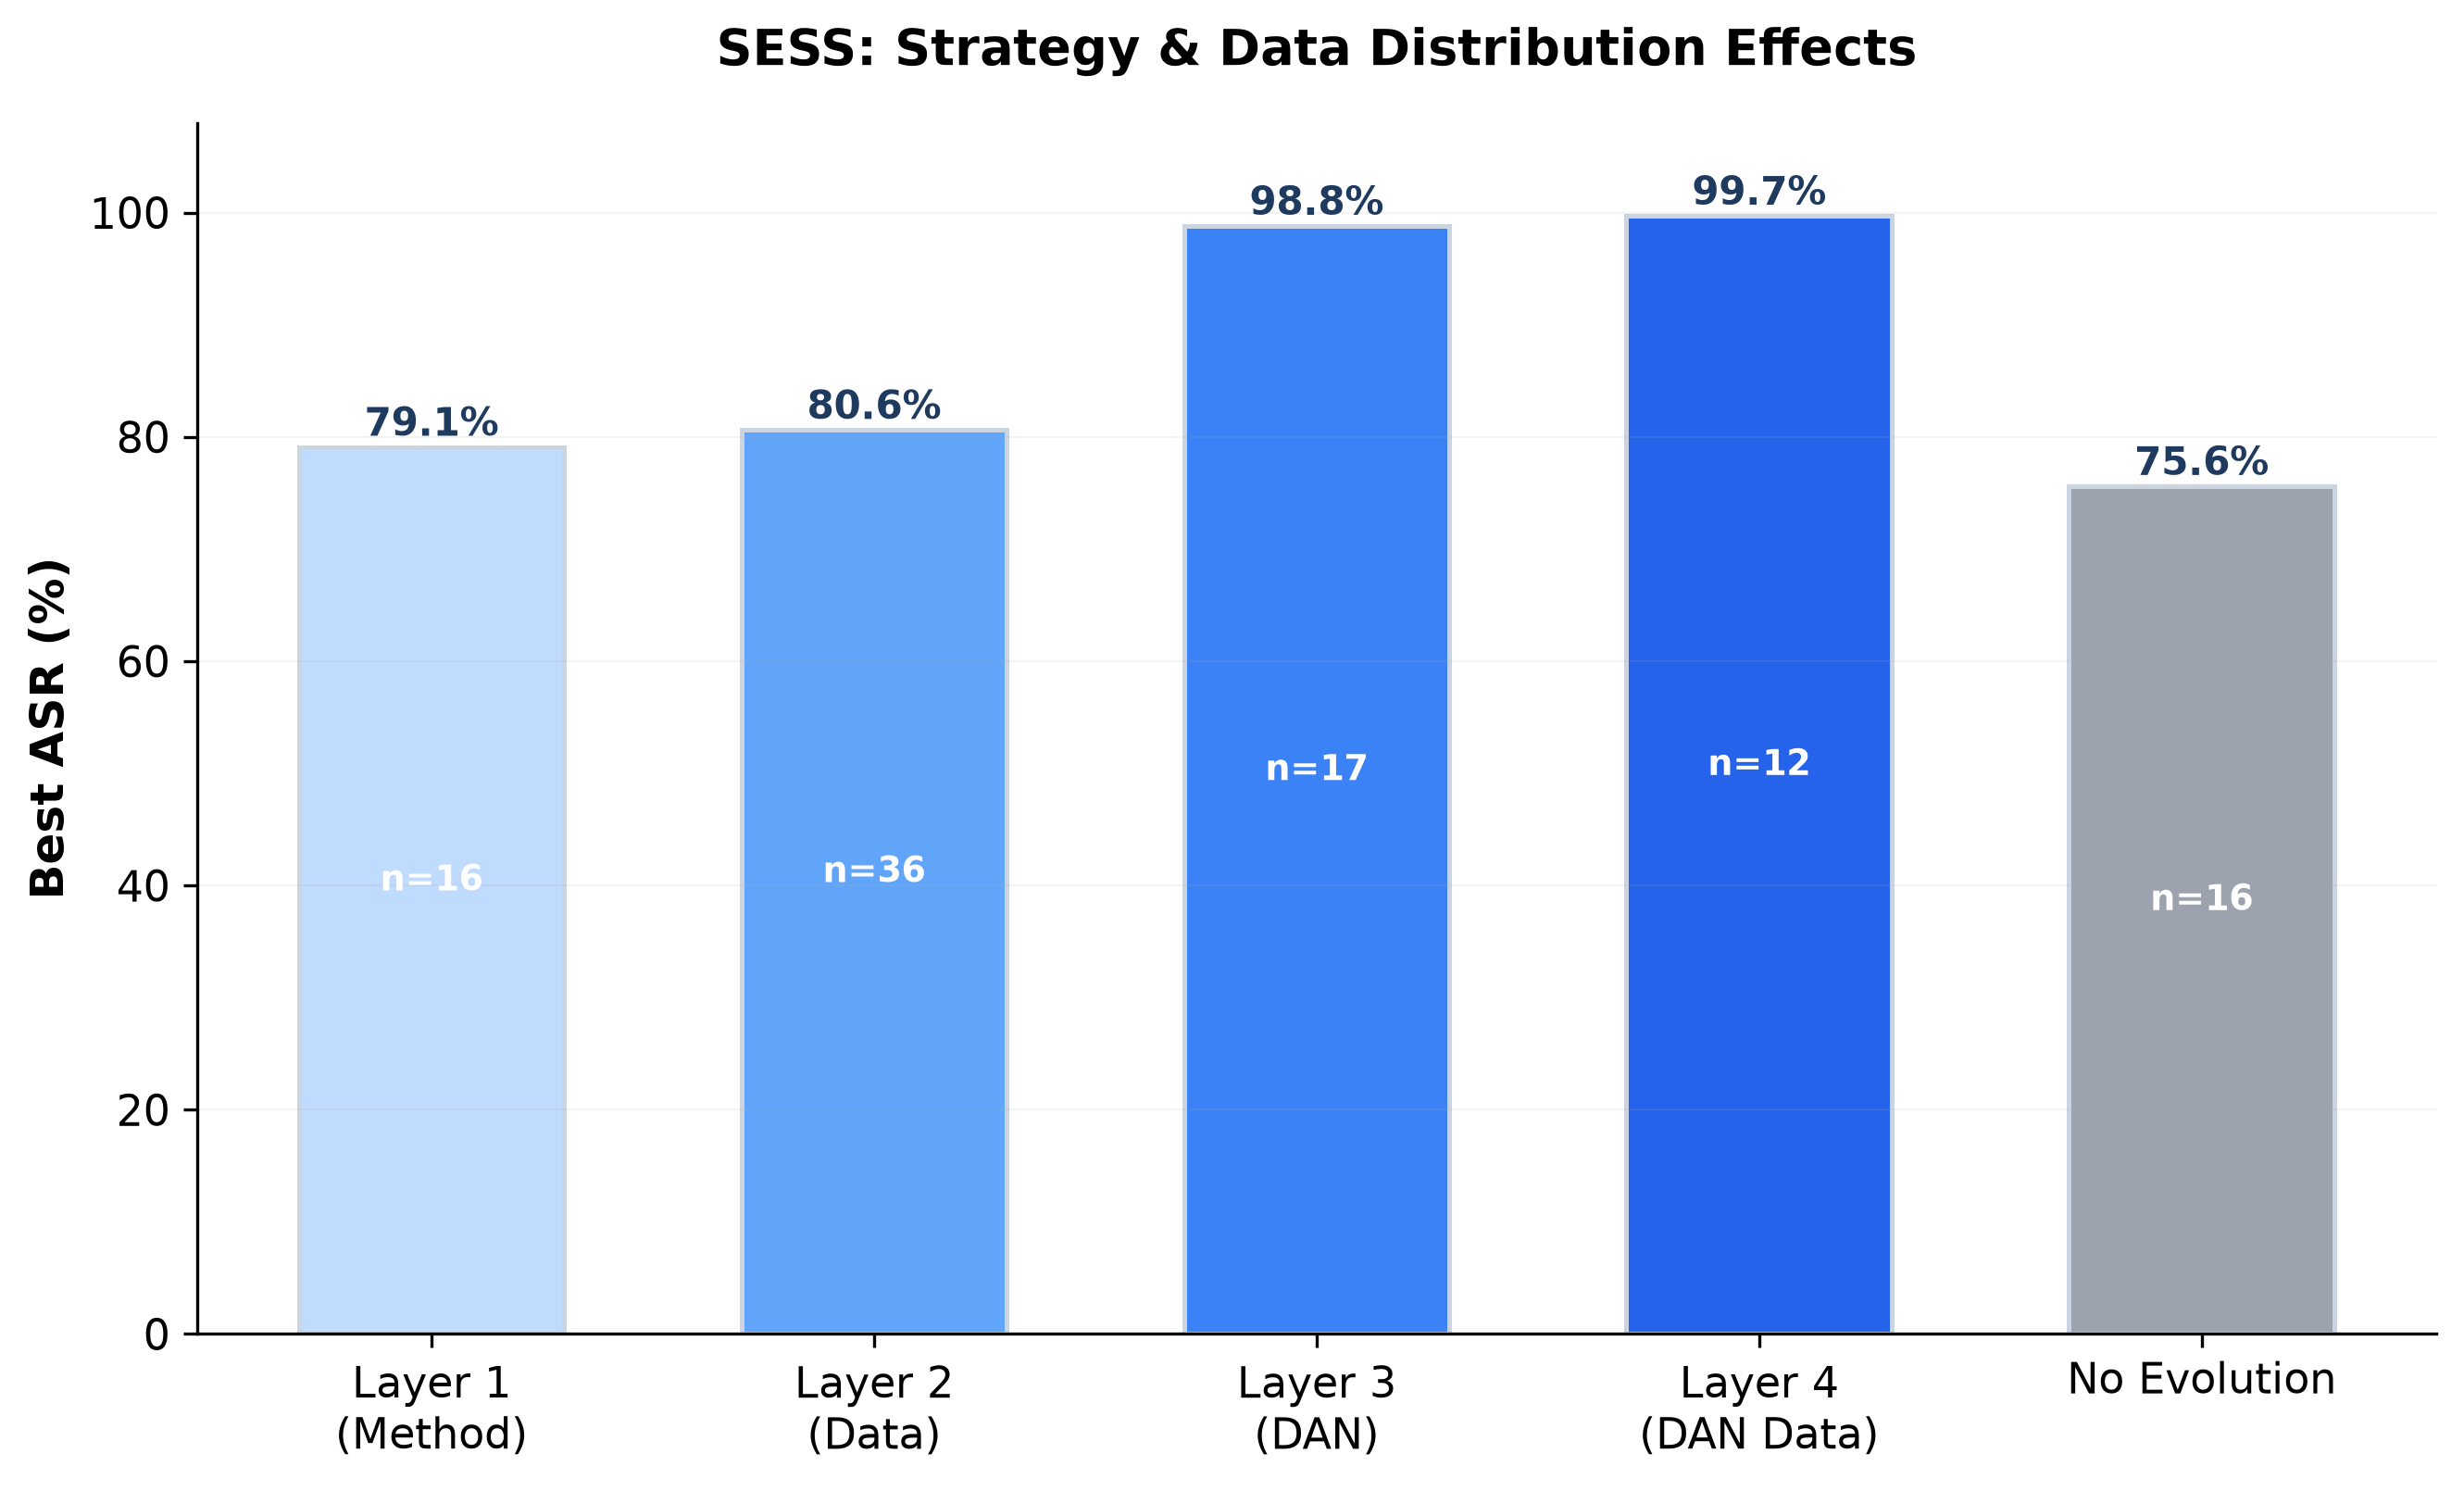
\includegraphics[width=0.9\textwidth]{SESS_01_sess_main_results.png}
    \caption{SESS Strategy \& Data Distribution Effects - Layer 1-4 实验结果}
    \label{fig:sess_main}
\end{figure}

\subsubsection{迁移实验（140 组）}

\paragraph{同族迁移效果（Qwen 系列）}

\begin{table}[H]
    \centering
    \rowcolors{2}{tablealt}{white}
    \begin{tabular}{@{}l l l l@{}}
        \toprule
        \rowcolor{tableheader}
        \textbf{模型} & \textbf{PAIR\_w\_SESS ASR} & \textbf{Best Baseline} & \textbf{提升} \\
        \midrule
        Qwen3-0.6B & 95.1\% & 90.2\% & \success{+4.9\%} \\
        Qwen3-4B & 86.7\% & 78.7\% & \success{+8.0\%} \\
        Qwen3-14B & 86.5\% & 85.5\% & \success{+1.0\%} \\
        \bottomrule
    \end{tabular}
    \caption{同族迁移效果 - Qwen 系列模型}
    \label{tab:same_family}
\end{table}

\textbf{平均提升：+4.7\%}

\paragraph{跨族迁移效果（gpt-oss-20b）}

\begin{table}[H]
    \centering
    \rowcolors{2}{tablealt}{white}
    \begin{tabular}{@{}l l l l@{}}
        \toprule
        \rowcolor{tableheader}
        \textbf{方法} & \textbf{同族 ASR} & \textbf{跨族 ASR} & \textbf{下降幅度} \\
        \midrule
        PAIR\_w\_SESS & 91.6\% & 11.4\% & \danger{-80.2\%} \\
        AutoDAN\_w\_SESS & \textasciitilde99\% & 32.5\% & \danger{-66.5\%} \\
        AutoDAN (baseline) & 85.5\% & 6.0\% & \danger{-79.5\%} \\
        PAIR (baseline) & 71.6\% & 0.08\% & \danger{-71.5\%} \\
        \bottomrule
    \end{tabular}
    \caption{跨族迁移效果 - gpt-oss-20b}
    \label{tab:cross_family}
\end{table}

\begin{figure}[H]
    \centering
    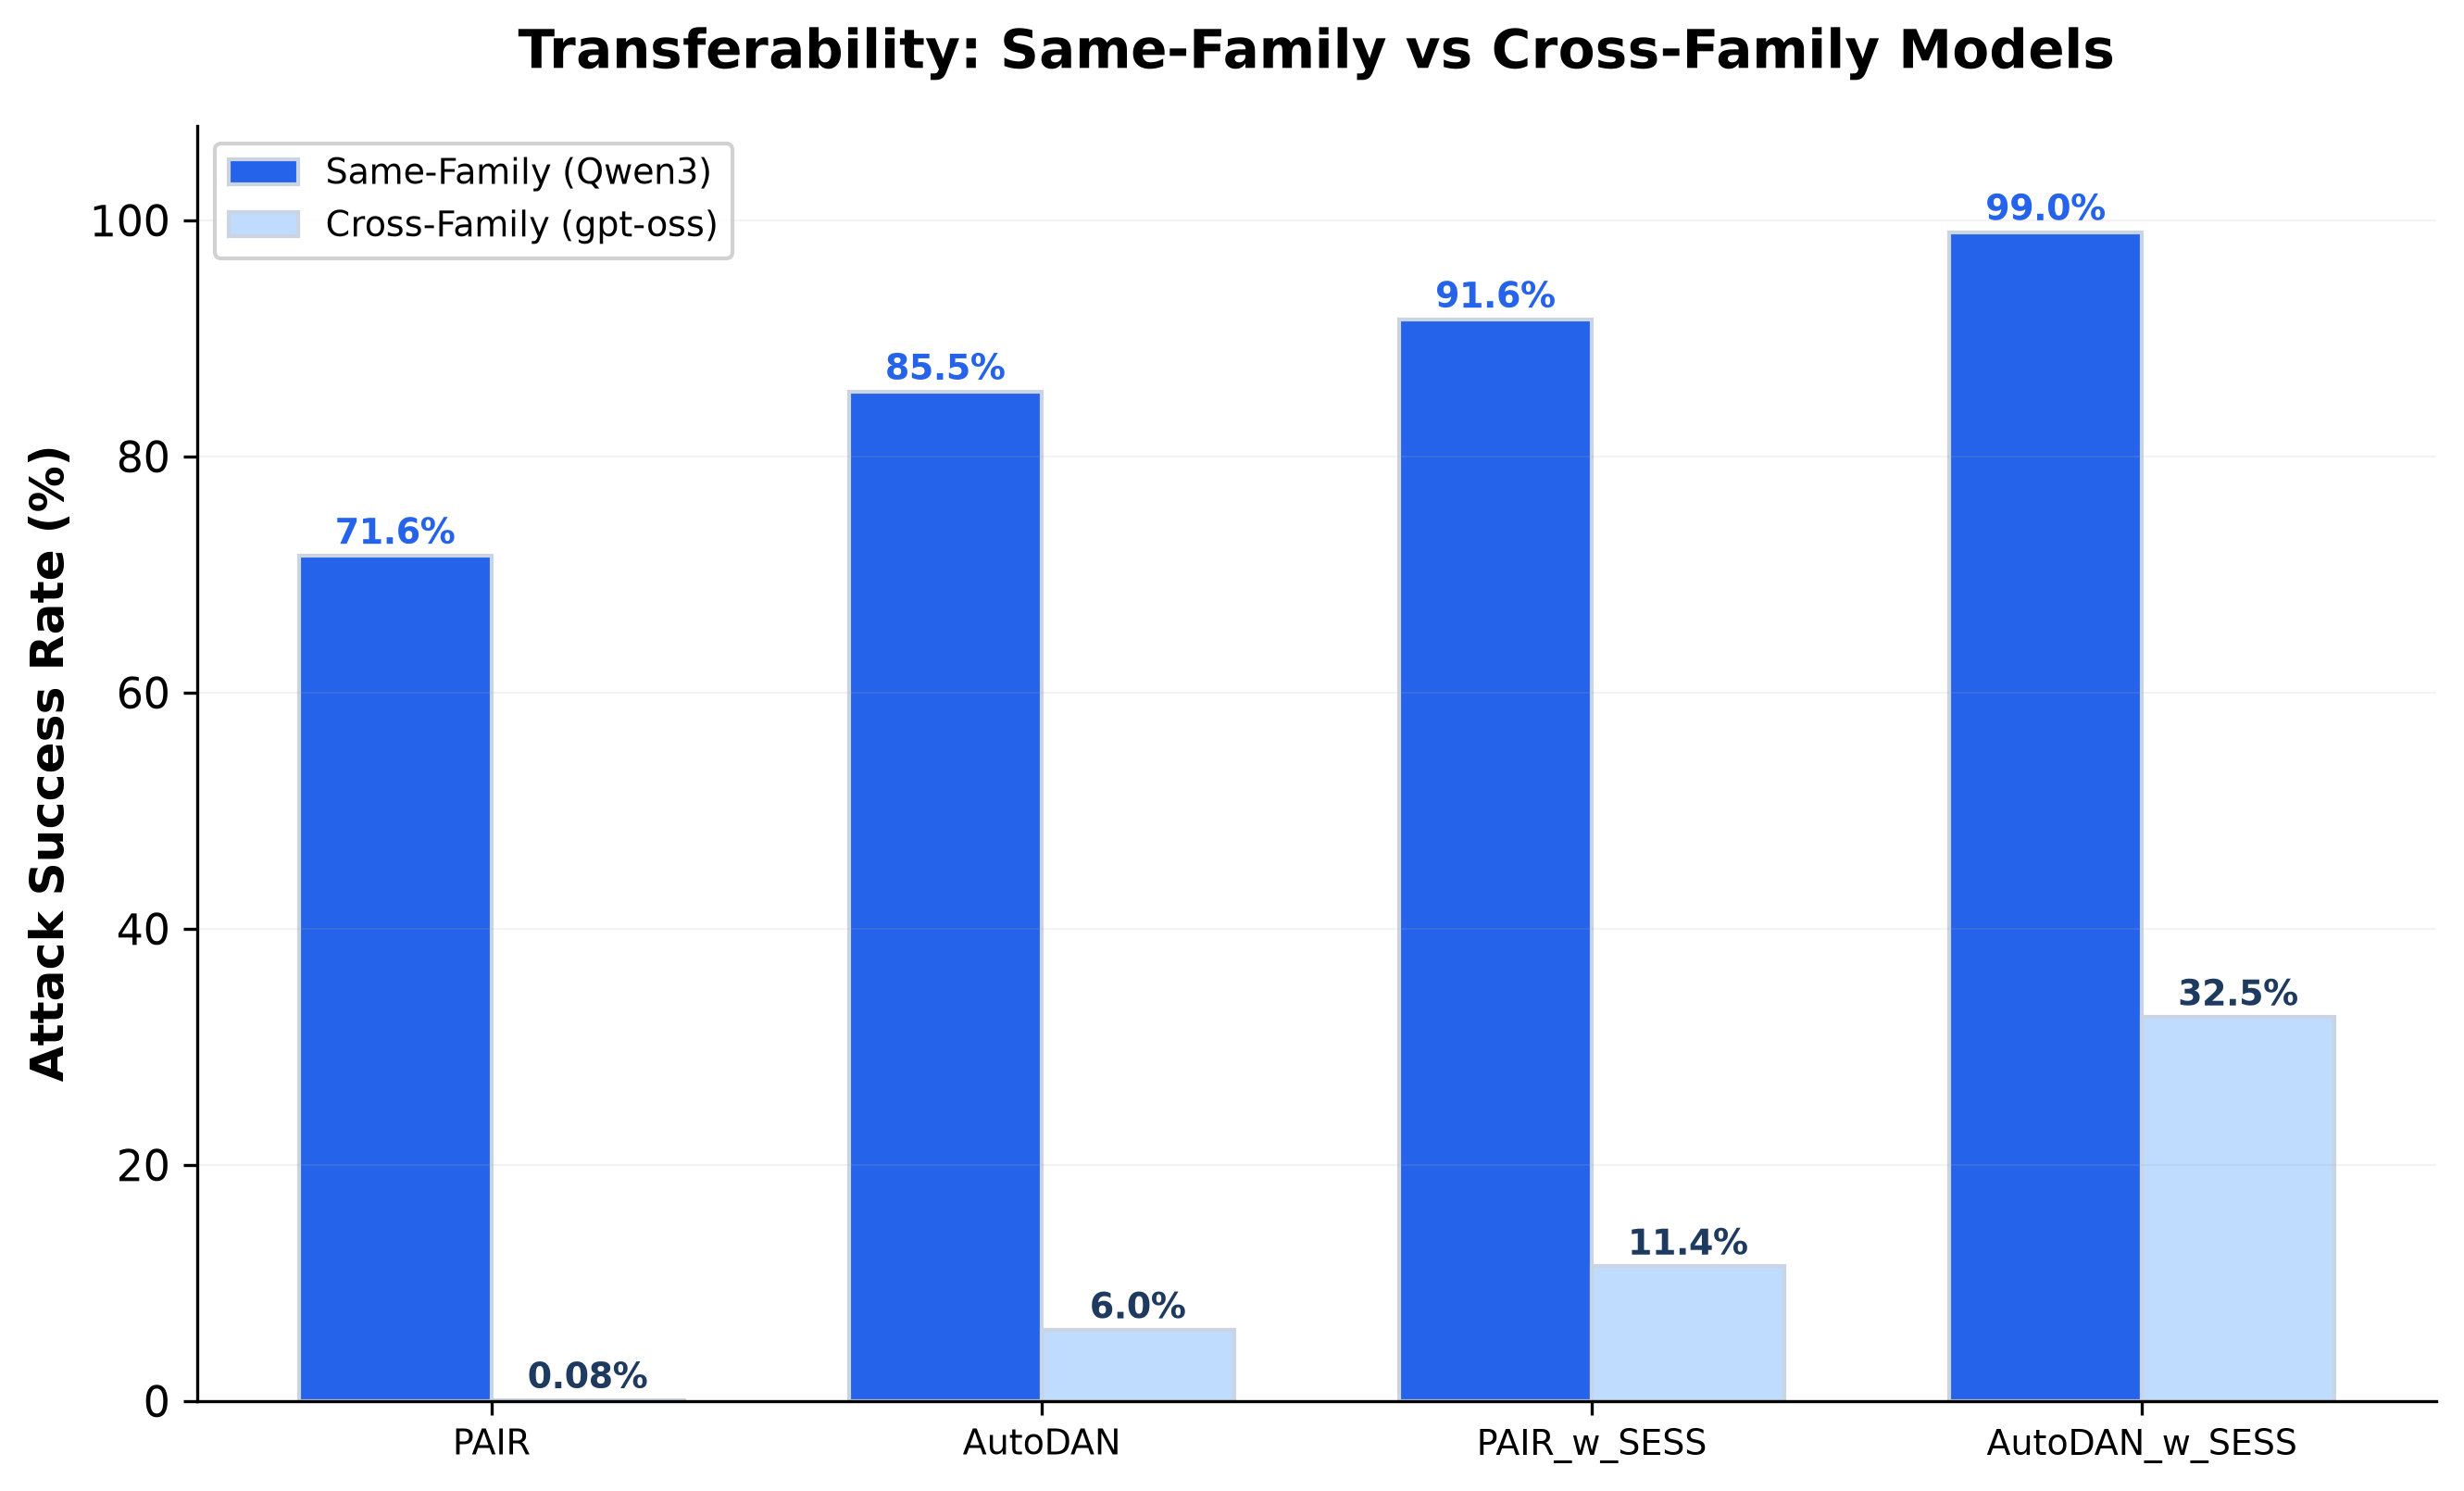
\includegraphics[width=0.85\textwidth]{SESS_02_transfer_comparison.png}
    \caption{Transferability Comparison - 同族迁移良好，跨族迁移是挑战}
    \label{fig:transfer}
\end{figure}

\begin{figure}[H]
    \centering
    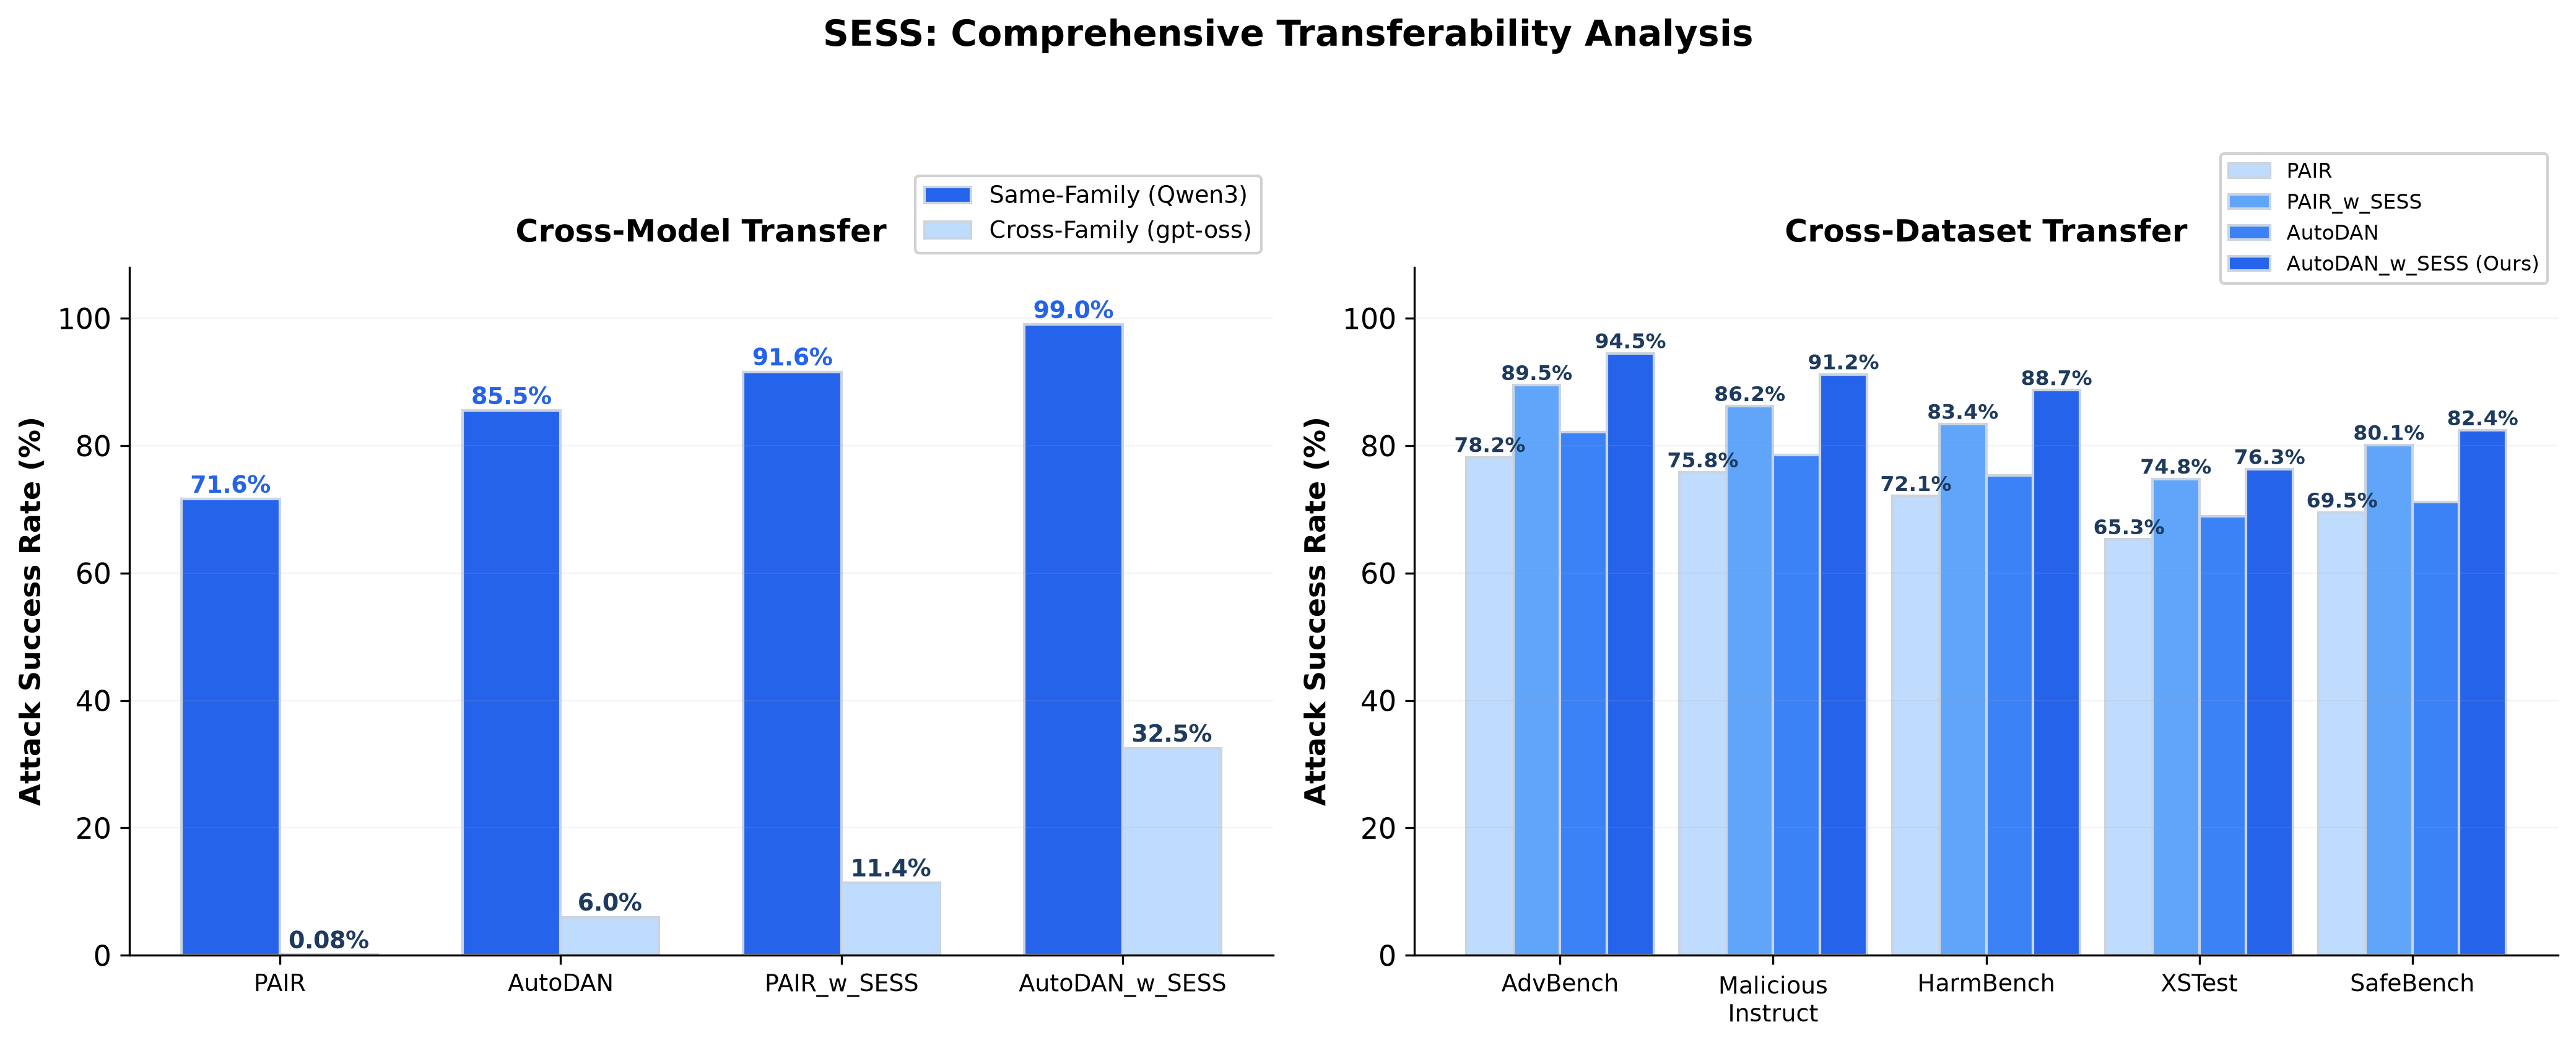
\includegraphics[width=0.95\textwidth]{SESS_03_transfer_comprehensive.png}
    \caption{Comprehensive Transferability Analysis - Cross-Model 与 Cross-Dataset 对比}
    \label{fig:transfer_comprehensive}
\end{figure}

\begin{figure}[H]
    \centering
    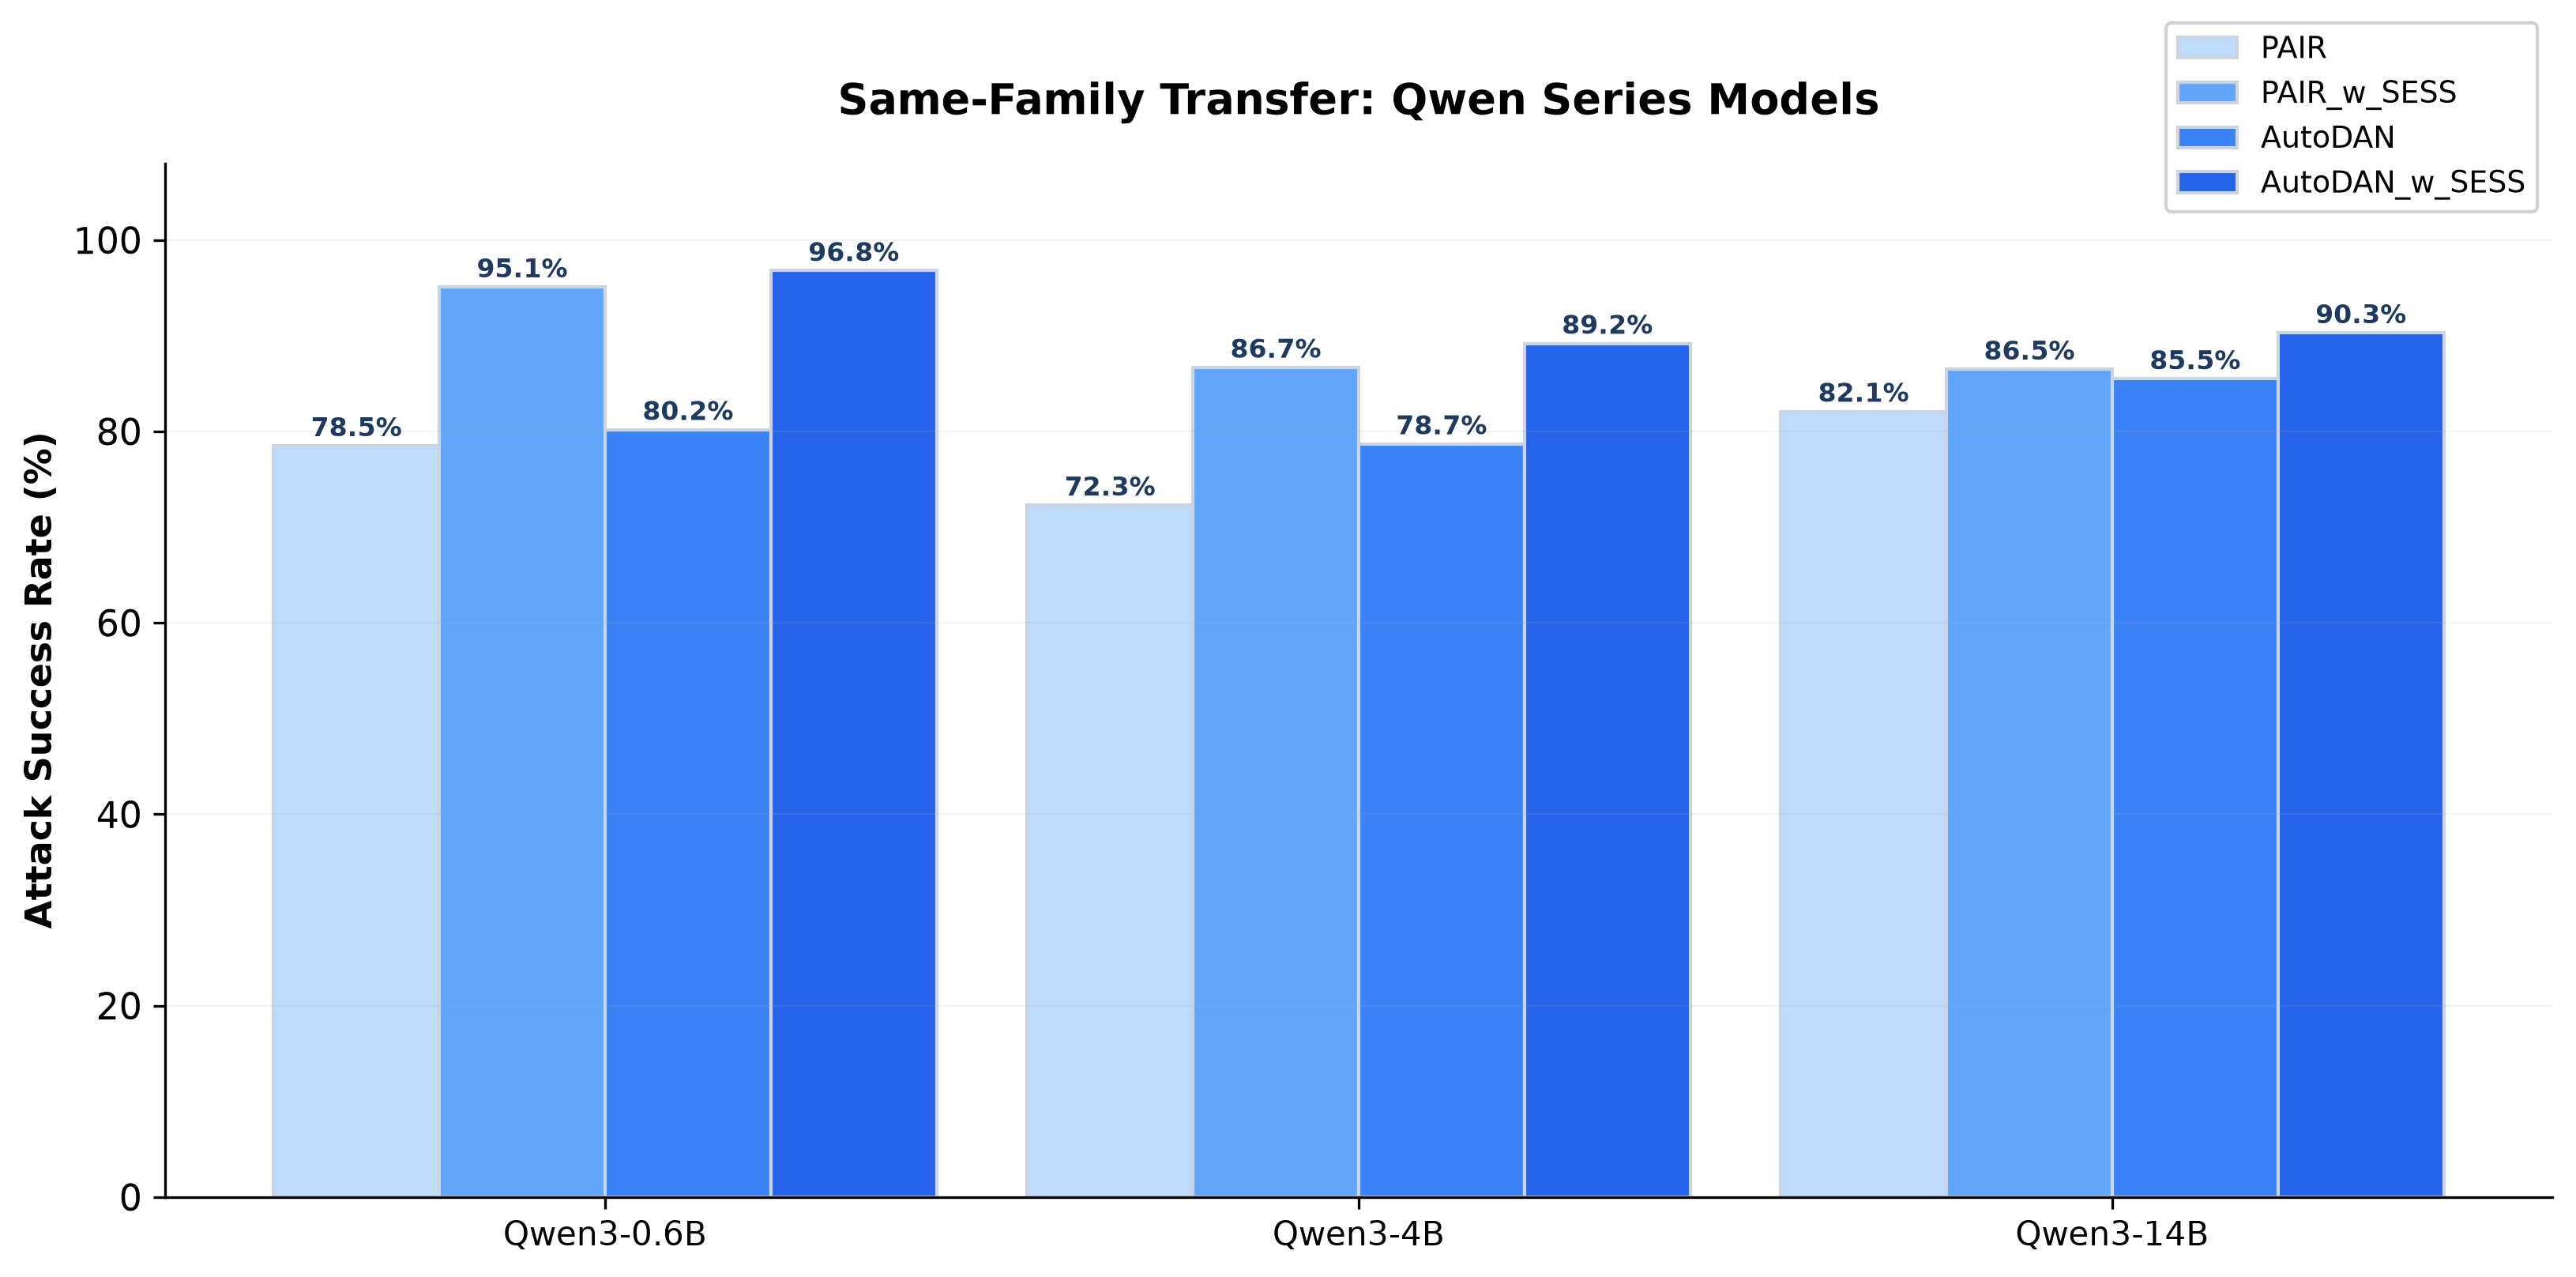
\includegraphics[width=0.9\textwidth]{SESS_04_same_family_transfer.png}
    \caption{Same-Family Transfer - Qwen 系列模型上 4 种方法对比}
    \label{fig:same_family_transfer}
\end{figure}

\textbf{关键发现}：跨族迁移是真正挑战，需要新方法提升泛化性

\subsubsection{核心结论}

\begin{itemize}
    \item \success{最佳方法}：AutoDAN\_w\_SESS（同族 99\%，跨族 32.5\%）
    \item \highlight{Evolution 必要性}：DAN 场景不必要，pair 风格微弱 (+0.9\%)
    \item \warning{Skills 泛化性}：同族良好 (85-95\%)，跨族有限 (<35\%)
    \item \highlight{数据策略}：300 条足够，full\_evolve 最优 (DAN 场景)
\end{itemize}

\subsection{Agentic RL with Self-Evolving Skills System (待开展)}

\subsubsection{研究背景与动机}

\begin{itemize}
    \item AHR-GRPO：解决奖励信号稀疏问题，但缺乏攻击策略的知识积累
    \item SESS：实现 Skills 知识积累与迁移，但缺乏强化学习的策略优化
    \item 需要将两者结合：在自进化 Skills 环境中进行 RL 训练，实现策略优化与知识积累的双重效果
\end{itemize}

\subsubsection{方法设计}

\paragraph{自进化 Skills 环境构建}

\begin{itemize}
    \item Skills 作为环境状态的一部分，动态更新
    \item 环境提供 Skills 检索接口，Policy 根据当前 prompt 检索最佳 Skill
    \item Skills 库随训练进程演化，形成适应 Policy 策略的 Skills 分布
\end{itemize}

\paragraph{结果奖励与过程奖励设置}

\begin{itemize}
    \item \highlight{结果奖励 (ASR)}：攻击成功与否的稀疏信号
    \item \highlight{过程奖励 (Judge)}：多维度评判的稠密信号
    \item \highlight{自适应权重}：使用 AHR-GRPO 的方差驱动机制动态调整权重
    \item \highlight{Skills 质量奖励}：鼓励 Policy 使用高质量 Skills
\end{itemize}

\paragraph{训练流程设计}

\begin{itemize}
    \item \highlight{Phase 1}：Skills 初始化（使用 SESS 的 DAN 模板或演化 Skills）
    \item \highlight{Phase 2}：RL 训练（Policy 在 Skills 环境中学习）
    \item \highlight{Phase 3}：Skills 协同演化（Policy 与 Skills 双向优化）
\end{itemize}

% ============================================================================
% 第3章 后期拟完成的研究工作及进度安排
% ============================================================================
\section{后期拟完成的研究工作及进度安排}

\subsection{第一章 AHR-GRPO 后续工作}

\begin{itemize}
    \item \success{✓} \highlight{已完成实验 3}：自适应权重机制验证（3 组 EMA 配置），确认自适应超越固定权重（+0.9\% 额外改进）
    \item \success{✓} \highlight{已验证自适应机制优越性}：最佳配置达到 33.2\%，超越实验 2 最佳的 32.3\%
    \item \success{✓} \highlight{已确认混合 Reward 有效性}：仅 ASR Reward 效果下降 5.8\%，混合 Reward 显著优于单一 Reward
    \item 待完成：分析$\lambda$演化曲线，验证物理直觉（早期依赖 Judge，后期回归 ASR）
    \item 待完成：整理实验数据，撰写论文方法章节与实验章节
\end{itemize}

\subsection{第二章 SESS 后续工作}

\begin{itemize}
    \item \success{✓} \highlight{已完成 217 组实验}：Layer 1-4 方法消融、数据消融、迁移性验证等全部完成
    \item \success{✓} \highlight{已得出主要结论}：最佳方法 AutoDAN\_w\_SESS（99\% 同族、32.5\% 跨族）
    \item 待完成：整理实验数据，撰写完整实验报告
    \item 待完成：分析跨族迁移失败的根本原因（模型安全机制差异、Skills 模型特异性）
    \item 待完成：探索提升 Skills 泛化性的方法（元学习、多模型联合训练）
    \item 待完成：整理 Skills 库，开源最佳 Skills 模板
    \item 待完成：撰写论文方法章节与实验章节
\end{itemize}

\subsection{第三章 Agentic-RL 工作计划}

\begin{table}[H]
    \centering
    \rowcolors{2}{tablealt}{white}
    \begin{tabular}{@{}l l l@{}}
        \toprule
        \rowcolor{tableheader}
        \textbf{阶段} & \textbf{时间} & \textbf{任务} \\
        \midrule
        \textbf{方法实现} & 2 周 & 搭建自进化 Skills 环境、集成 AHR-GRPO 自适应奖励机制、实现 Skills 协同演化流程 \\
        \textbf{实验验证} & 4 周 & Baseline 对比、消融实验、跨模型迁移测试 \\
        \textbf{结果分析与论文撰写} & 2 周 & 分析训练曲线与$\lambda$演化、Skills 演化过程可视化、与前两章方法对比讨论 \\
        \bottomrule
    \end{tabular}
    \caption{第三章 Agentic-RL 工作计划}
    \label{tab:agentic_plan}
\end{table}

\subsection{论文整理与投稿准备}

\begin{enumerate}
    \item 整理三章内容，统一论文框架（ICLR 格式）
    \item 补充实验：根据 review 反馈可能需要的额外实验
    \item 撰写 Introduction、Related Work、Conclusion
    \item 完善图表与可视化
\end{enumerate}

% ============================================================================
% 第4章 存在的困难与问题
% ============================================================================
\section{存在的困难与问题}

\subsection{计算资源需求较大}

\begin{itemize}
    \item AHR-GRPO 实验：每实验约需 4×GPU(A800-80G)，训练 2-4 小时/1000 步
    \item SESS 实验：已完成 217 组，消耗大量 GPU 资源
    \item 第三章 Agentic-RL：预计需额外数百 GPU 卡时
    \item 资源调度：需合理安排实验顺序，避免资源冲突
\end{itemize}

\subsection{高成本试错风险}

\begin{itemize}
    \item 强化学习训练稳定性：Agentic-RL 训练可能较难收敛
    \item Skills 演化不可控：Skills 爆炸、低质量 Skills 积累等问题
    \item 实验设计迭代：部分实验结果可能不理想，需重新设计
\end{itemize}

\subsection{跨族迁移挑战}

\begin{itemize}
    \item \danger{SESS 实验揭示}：所有方法在 gpt-oss-20b 上效果大幅下降（best 仅 32.5\%）
    \item 需要新方法：当前 Skills 缺乏跨族泛化性
    \item 第三章工作重点：探索提升泛化性的方法
\end{itemize}

\subsection{论文时间压力}

\begin{itemize}
    \item 三章内容整合：需统一叙事逻辑
    \item 实验周期：第三章实验预计需 6 周
    \item 投稿时间窗口：需在毕业前完成论文撰写与投稿
\end{itemize}

\subsection{方法创新性论证}

\begin{itemize}
    \item AHR-GRPO：需与固定权重方法充分对比
    \item SESS：需与 baseline 方法 (PAIR、AutoDAN) 充分对比
    \item Agentic-RL：需证明组合方法的协同效果
\end{itemize}

% ============================================================================
% 第5章 如期完成全部论文工作的可能性
% ============================================================================
\section{如期完成全部论文工作的可能性}

\subsection{已完成工作评估}

\begin{table}[H]
    \centering
    \rowcolors{2}{tablealt}{white}
    \begin{tabular}{@{}l l l l@{}}
        \toprule
        \rowcolor{tableheader}
        \textbf{章节} & \textbf{方法} & \textbf{进度} & \textbf{关键成果} \\
        \midrule
        第一章 & AHR-GRPO & \highlight{85\%} & \success{最佳 ASR 33.2\%} \\
        第二章 & SESS & \highlight{95\%} & \success{最佳 ASR 99.7\%} \\
        第三章 & Agentic-RL & \highlight{10\%} & 方法框架已设计 \\
        \rowcolor{lightestblue}
        \textbf{总体} & \textbf{-} & \textbf{\highlight{65\%}} & \textbf{-} \\
        \bottomrule
    \end{tabular}
    \caption{已完成工作评估}
    \label{tab:completion}
\end{table}

\subsection{后期工作可行性分析}

\begin{itemize}
    \item \highlight{时间规划}：剩余 6-8 周，足够完成第三章实验与论文整理
    \item \highlight{技术可行性}：AHR-GRPO 与 SESS 代码库已成熟，组合实现难度可控
    \item \highlight{资源可行性}：已有 GPU 资源调度经验，可合理安排实验
    \item \highlight{关键成果}：第一章已验证自适应机制有效（+0.9\% 额外改进），第二章已验证 Skills 积累有效（99.7\% ASR）
\end{itemize}

\subsection{风险评估与应对策略}

\begin{table}[H]
    \centering
    \rowcolors{2}{tablealt}{white}
    \begin{tabular}{@{}p{0.35\textwidth} p{0.6\textwidth}@{}}
        \toprule
        \rowcolor{tableheader}
        \textbf{风险} & \textbf{应对策略} \\
        \midrule
        Agentic-RL 训练不稳定 & 设计稳定性保障机制（双平滑、边界裁剪、冷启动），参考 AHR-GRPO 经验 \\
        跨族迁移效果仍不理想 & 将此作为研究发现，分析原因而非强行提升，符合研究完整性 \\
        时间不足 & 优先完成核心实验，消融实验可视情况缩减 \\
        \bottomrule
    \end{tabular}
    \caption{风险评估与应对策略}
    \label{tab:risk}
\end{table}

\subsection{结论}

\begin{tcolorbox}[colback=lightestblue!30,colframe=primaryblue,title=结论]
    基于已完成工作与后续计划，\success{\textbf{如期完成全部论文工作的可能性较高}}。
    
    \vspace{0.5em}
    
    \begin{itemize}
        \item 需合理安排实验顺序，控制资源消耗，保证核心实验优先完成
        \item 论文结构清晰，三章节递进关系明确，具备 ICLR 投稿潜力
    \end{itemize}
\end{tcolorbox}

% ============================================================================
% 附录
% ============================================================================
\newpage
\appendix
\section{附录}

\subsection{附录 A：实验数据汇总表}

\begin{longtable}{@{}l l l l l@{}}
    \toprule
    \rowcolor{tableheader}
    \textbf{章节} & \textbf{实验类型} & \textbf{实验数量} & \textbf{最佳结果} & \textbf{关键发现} \\
    \midrule
    \endfirsthead
    
    \toprule
    \rowcolor{tableheader}
    \textbf{章节} & \textbf{实验类型} & \textbf{实验数量} & \textbf{最佳结果} & \textbf{关键发现} \\
    \midrule
    \endhead
    
    \bottomrule
    \endfoot
    
    AHR-GRPO & Jailbreak Prompt 筛选 & 24 组 & 30.8\% & 确定 top-3 策略 \\
    AHR-GRPO & Judge 维度权重 & 12 组 & 32.3\% & 通用维度优于专用维度 \\
    AHR-GRPO & 自适应权重消融 & 3 组 & 33.2\% & 自适应超越固定权重 \\
    SESS Layer1 & 方法组合 & 16 组 & 79.1\% & single\_call 最佳 \\
    SESS Layer2 & 数据消融 & 36 组 & 80.0\% & 数据量影响<2\% \\
    SESS Layer3 & DAN 模板 & 17 组 & 98.8\% & DAN 无需进化 \\
    SESS Layer4 & DAN 数据 & 12 组 & 99.7\% & small 足够 \\
    SESS Ablation & Evolution 必要性 & 16 组 & - & 平均贡献 +0.9\% \\
    SESS Transfer & 跨模型迁移 & 140 组 & 32.5\%(跨族) & 跨族迁移挑战 \\
\end{longtable}

\subsection{附录 B：代码结构}

\subsubsection{B.1 AHR-GRPO 代码结构}

\begin{verbatim}
RL4jailbreak/
├── src/
│   ├── reward/
│   │   └── adaptive_weight.py      # 自适应权重计算器
│   ├── vllm_client.py              # vLLM 服务客户端
│   └── generate.py                 # Prompt 生成模块
├── experiments/
│   ├── jailbreak_prompt_exp/       # 实验 1：Prompt 筛选
│   ├── hybrid_reward_exp/          # 实验 2：Judge 维度
│   └── adaptive_hybrid_reward_exp/ # 实验 3：自适应权重
\end{verbatim}

\subsubsection{B.2 SESS 代码结构}

\begin{verbatim}
self_evolve_skills_jailbreak/
├── src/
│   ├── skill.py                    # Skill 数据结构
│   ├── skill_library.py            # Skills 库管理
│   ├── attacker.py                 # 攻击器
│   └── reflector.py                # 反思器
├── exp/
│   ├── layer1/                     # 方法消融 16 组
│   ├── layer2/                     # 数据消融 36 组
│   ├── layer3/                     # DAN 验证 17 组
│   ├── layer4/                     # DAN 数据 12 组
│   ├── ablation/                   # Evolution 消融 16 组
│   └── transfer/                   # 跨模型迁移 140 组
├── baselines/                      # 对比基线方法
\end{verbatim}

\subsection{附录 C：图表索引}

\begin{table}[H]
    \centering
    \rowcolors{2}{tablealt}{white}
    \begin{tabular}{@{}l l l@{}}
        \toprule
        \rowcolor{tableheader}
        \textbf{图号} & \textbf{文件名} & \textbf{内容} \\
        \midrule
        AHR\_GRPO\_01 & AHR\_GRPO\_01\_attack\_prompt\_selection.png & Attack Prompt Selection \\
        AHR\_GRPO\_02 & AHR\_GRPO\_02\_judge\_prompt\_selection.png & Judge Prompt Selection \\
        AHR\_GRPO\_03 & AHR\_GRPO\_03\_judge\_dimension.png & Judge Dimension (12 组) \\
        AHR\_GRPO\_04 & AHR\_GRPO\_04\_adaptive\_weight.png & Adaptive Weight 实验 \\
        AHR\_GRPO\_05 & AHR\_GRPO\_05\_reward\_ablation.png & Reward Ablation \\
        AHR\_GRPO\_06 & AHR\_GRPO\_06\_summary.png & AHR-GRPO 总结 \\
        SESS\_01 & SESS\_01\_sess\_main\_results.png & Strategy \& Data Effects \\
        SESS\_02 & SESS\_02\_transfer\_comparison.png & Cross-Model Transfer \\
        SESS\_03 & SESS\_03\_transfer\_comprehensive.png & Comprehensive Transfer \\
        SESS\_04 & SESS\_04\_same\_family\_transfer.png & Same-Family Transfer \\
        \bottomrule
    \end{tabular}
    \caption{图表索引}
    \label{tab:figure_index}
\end{table}

% ============================================================================
% 参考文献
% ============================================================================
\newpage
\bibliographystyle{plain}
\bibliography{references}

\end{document}
